\documentclass[a4paper, 12pt]{paper}

\usepackage{BMETeX_BSc}
\usepackage{fancyvrb}
\usepackage{tocloft}
\usepackage{algorithm}
\usepackage{algpseudocode}
\usepackage{multirow}
\newlength\longest
\renewcommand{\tableshortname}{Table}
\makeatletter
\def\BState{\State\hskip-\ALG@thistlm}
\renewcommand{\fnum@figure}{Figure \thefigure}
\makeatother

\VerbatimFootnotes
\bibliographystyle{IEEEtranN}

\begin{document}

\pagenumbering{Roman} % Roman numbering
\begin{center}
    \begin{figure}[!h]
        \centering
        
\includegraphics[width=0.6\linewidth]{bme_logo_nagy.pdf}
    \end{figure}
    \large\textsc{Budapest University of Technology and Economics\\
        Dep. of Control for Transportation
        and Vehicle Systems}
\end{center}
\thispagestyle{empty}
{\centering
    \vspace*{\stretch{0.2}}

    {\LARGE\textsc{Domonkos Csuzdi}

        \LARGE{Students' Scientific Conference Report}}

    {\Large\textbf{\\Daum--Huang Filter for LiDAR-based Mobile Robot Localization}}\\

    \vspace*{\stretch{0.2}}}

\begin{flushleft}
    \begin{minipage}{0.3\linewidth}
        \large{Consultant}:\\
        \forceindent \textit{Olivér Törő}\\
        \forceindent PhD candidate
    \end{minipage}
\end{flushleft}


\vspace*{\stretch{0.5}}

\begin{center}
    {\Large\textsc{Budapest, }2021 }
\end{center}
\vspace*{\stretch{0.1}}
\newpage
\thispagestyle{empty}
\newpage
\section*{Acknowledgement}
This work has been supported by the Hungarian Government and co-financed by the European Social Fund. (Contract Identifier: EFOP-3.6.3-VEKOP-16-2017-00001. Talent management in autonomous vehicle control technologies.) Their support is gratefully acknowledged.
I would also like to thank Dániel Doba for his help with ROS, and his much appreciated insights.
I am most grateful to my consultant, Olivér Törő, who was always available for valuable discussions.
% TODO thanks to Olivér and Dani (ROS)
\clearpage
\tableofcontents
\pagebreak
\pagenumbering{arabic}
\pagestyle{fancy}
\section{Introduction}

Even in antiquity, localization -- based on various reference points -- played a significant role, especially in the case of pelagic navigation. In the Age of Discovery, the so-called dead reckoning method served as a particularly handy method of position estimation. In this case, localization merely consisted of approximating the traveled distance by only measuring speed, the direction of movement, and elapsed time. Nowadays the de facto standard is the Global Navigation Satellite System (GNSS), however, it behaves poorly (or even not functional) in shielded environments. If for example, an autonomous vehicle performs a parking task in a garage, localization is often performed by different state estimation algorithms.

Such algorithm is the Kalman Filter, which serves as an optimal estimator for linear, Gaussian, dynamical systems. However, in reality, both linearity and Gaussian nature are often violated. To overcome these effects, various nonlinear filters, such as the Extended Kalman filter (EKF) or different particle filter-based algorithms can be applied instead. One prominent alternative is the so-called Daum–Huang filter (DHF), which development was mainly motivated by the shortcomings of particle filters, and was originally designed for satellite localization.

The main goal of this report is to propose an improved
localization algorithm for a mobile robot with an
equipped LiDAR sensor, based on the DHF.
Nowadays, one of the most popular localization algorithm
for such setup is the Adaptive Monte Carlo Localization, which is based on a particle filter.
As Daum--Huang filters are mainly developed to overcome important shortcomings of particle
filters, they may be able to also outperform particle filters in a low-dimensional mobile robot
localization task.

In order to implement the sought localization algorithm, first, certain prerequisites
have to be introduced. In Section 2, the localization task is described in more detail,
followed by the basic structure of the TurtleBot3 mobile robot, along with its available sensors.
As the environment representation and the motion model of the robot are closely related to the equipped sensors, they are also discussed in this section.

Besides the motion model, another existential part of localization is the measurement model.
To suit the DHF algorithm, a newly proposed measurement model by Dantanarayana et al. in \cite{Dantanarayana2013} is utilized and detailed in section 3. Their method provides an implicit
measurement equation which is not suitable for the DHF-based localization in scope, as it
requires an explicit form. As a solution, a small addition is proposed in this report,
which enables the use of an implicit measurement equation.

The extended Kalman Filter (EKF) is directly required for the implemented Daum--Huang filter variant, therefore the Kalman filters are discussed in Subsection 4.1.
As Daum--Huang filters are closely related to particle filters, a brief overview is provided
in Subsection 4.3 through the examination of the bootstrap particle filter. This subsection also contains the description of the AMCL algorithm. Finally, the Daum--Huang filters are discussed in Subsection 4.4, along with the exact flow variant, as it is going to serve as the base for the
proposed localization algorithm, which pseudocode is provided in Subsection 4.5.


In Section 5, the performance of three localization algorithms is going to be tested:
the EKF-based localization  by Dantanarayana et al. \cite{Dantanarayana2016},
the EDH-based localization  algorithm proposed in this report,
and the Adaptive Monte Carlo Localization (AMCL)~\cite{AMCLROS2002}.
Their estimation errors are compared in a simulated environment by the Gazebo simulator and the Robot Operating System.

The report concludes with a summary in Section 6.



\pagebreak
\section{Hardware and Corresponding Models for Localization}
\subsection{Formulation of the Localization Task}

During localization the main goal is to determine the coordinate transformation between the local coordinate system of the robot,
and a given global frame.
For most of the problems a Global Navigation Satellite System (GNSS), like GPS provides
this information.
In an ideal world the GPS data is precise and reliable, making state estimation based localization algorithms almost unnecessary.
However, it is well known that global positioning by satellites cannot be performed in environments
where the satellite signal is not available, or not strong enough
(for example indoors), and even outdoors, the provided precision is often not sufficient.

To overcome these deficiencies, different state estimation algorithms are used to obtain the pose of the robot in the global frame.
Localization and mapping often goes hand in hand: localization without a map
(or some kind of a representation of the environment on which the global frame is defined),
and map creation without the information about the pose is hardly possible.
If one of them is assumed to be known, the task is much easier: localization, or mapping.
If both are sought after, the Simultaneous Localization and Mapping (SLAM) problem arises,
which is significantly harder than any of them separately.
In the scope of this report, only the localization task is addressed on a given (ground truth) map.

One possible way to achieve localization is the introduction of pose hypotheses.
By this the robot's belief of its pose is a probability distribution, instead of a crisp value~\cite{Thrun2005}.
Knowing the pose exactly is not feasible in a noisy real world environment.
For a localization task, two main hardware components are used: an effector which is responsible for moving the robot,
and an exteroceptive sensor, which is responsible for obtaining information about the surrounding environment (like a LiDAR, a sonar, or often a camera)
\cite{Siegwart2011}.
Both introduce errors and noise to the system which could be dealt with by the application of the probabilistic approach.
In the following, this modelling method is detailed.

Almost every state estimation (e.g. localization) algorithm is based on Bayesian filtering.
It serves as a theoretical foundation for these methods, thus could not be implemented as a
standalone filter.
A Bayes filter consists of two main parts which are iterated over time: prediction and update (see more in \cite{Thrun2005}).
These have the following forms (respectively):
\begin{align}
    \overline{bel}(\mathbf{x}_t) & = \int \underbrace{p(\mathbf{x}_t | \mathbf{x}_{t-1},\mathbf{u}_t)}_{\text{motion model}}bel(\mathbf{x}_{t-1})\mathrm{d}\mathbf{x}_{t-1}, \label{eq:bayes-predict} \\
    bel(\mathbf{x}_t)            & = \eta \underbrace{p(\mathbf{\mathbf{z}}_t | \mathbf{x}_t)}_{\text{meas. model}}\overline{bel}(\mathbf{x}_t),
\end{align}
where
\begin{align}\label{key}
    bel(\mathbf{x}_t)            & = p(\mathbf{x}_t|\mathbf{z}_{1:t},\mathbf{u}_{1:t}),                      \\
    \overline{bel}(\mathbf{x}_t) & = p(\mathbf{x}_t|\mathbf{z}_{1:t-1},\mathbf{u}_{1:t}) \label{eq:predbel}.
\end{align}
The notations are the following: $\mathbf{x}_t$ is the pose (position in 2D, and heading direction) at time $t$,
$\mathbf{u}_t$ is the input (control) vector at $t$, $\eta$ is a normalization constant from  Bayes' theorem,
$\mathbf{z}_t$ is the measurement at $t$, $(\cdot)_{1:t}$ denotes values from time $t = 1$ to $t$,
$bel(\mathbf{x}_t)$ is the belief (also called as posterior), and  $\overline{bel}(\mathbf{x}_t)$ is the predicted belief.

First, $\overline{bel}(\mathbf{x}_t)$ is calculated from the prior $bel(\mathbf{x}_{t-1})$, using the motion model.
This is a prediction, because only the kinematics are incorporated, not the measurements.
Then in the update part the measurement model is considered.
This corrigates (updates) the prediction by incorporating the observations.

However, these probability distributions and integrals cannot be calculated on their own.
Each distinct filter realizations address the solution of the Bayesian recursion differently:
the Kalman Filters use Gaussian distributions and their parametric descriptions to estimate the pose hypotheses,
while particle filters produce a more general numerical solution by representing an arbitrary distribution via particles.
The Daum--Huang filters also use particles, but describes their movement with the help of the Fokker--Planck equation.
These realizations are explained in greater detail in Section \ref{sec:state-estimators}.

\subsection{The Mobile Robot}\label{subsec:robot}
An important preliminary of localization is the introduction of the utilized hardware, the operating environment,
and their models.
In this subsection, the mobile robot itself is discussed, along with its relevant sensors,
followed by the environment representation where the robot has to be localized.

As an agent, the simulated version of ROBOTIS' TurtleBot3\footnote{https://www.robotis.us/turtlebot-3/} is used via Robot Operating System (ROS) and Gazebo.
This two-wheeled platform is widely used for educational and prototyping purposes due to its easy handling
and well developed simulational counterpart. Although it has many useful components, here only the LiDAR and the
differential drive are discussed due to their relevancy in the localization task.
Those and the robot itself can be seen in Figure~\ref{fig:turtlebot3-burger}.
\begin{figure}[htbp]
    \centering
    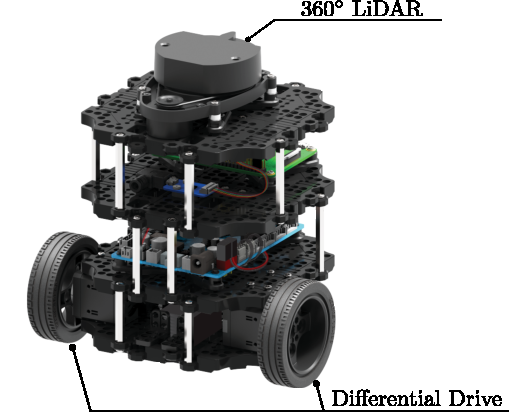
\includegraphics[width=0.5\linewidth]{turtlebot3_burger_components.pdf}
    \caption[]{ROBOTIS' TurtleBot3 Burger platform, with a mounted 360$^\circ$ LiDAR on top, and a differential drive (image source: www.robosklep.com).}
    \label{fig:turtlebot3-burger}
\end{figure}

The mounted 2D LiDAR provides range and angle measurements from the environment with $360^\circ$ field of view,
using the triangulation principle (for details, see \cite{Konolige2016}).
This particular model (LDS-01) has an angular resolution of $1^\circ$, detection range of $0.12-3.5$ m,
and accuracy (3$\sigma$) of $\pm$15 mm-s (to be precise, the precision is distance dependent, but this effect is not considered).
Invalid readings indicate out of range measurements. One full measurement is shown in Figure~\ref{fig:lidar-readings}.
\begin{figure}[htbp]
    \centering
    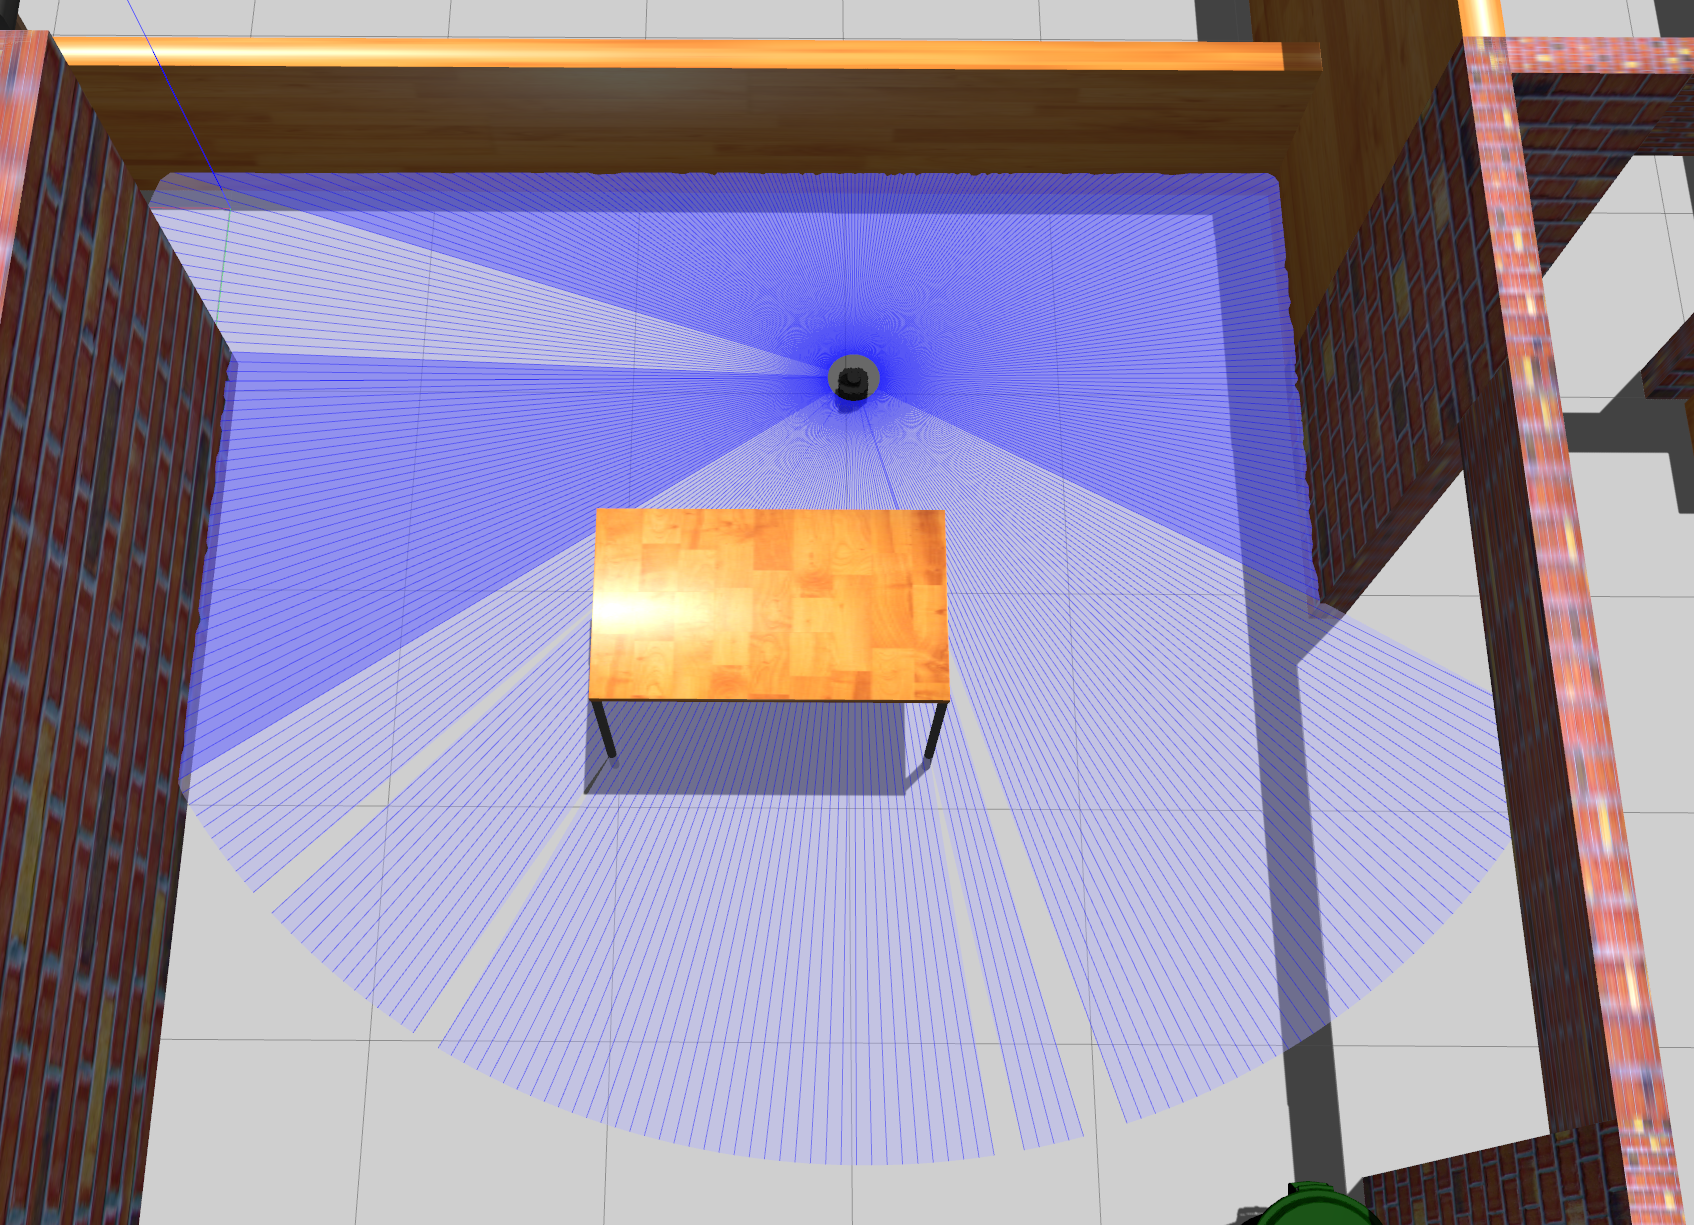
\includegraphics[width=0.6\linewidth]{lidar-visu.png}
    \caption{Visualized 2D LiDAR measurement of the TurtleBot3 in a house environment, using the Gazebo simulator.}
    \label{fig:lidar-readings}
\end{figure}

The platform has 2 independently-driven wheels, and one free turning wheel, which
makes it eligible to be modelled by differential drive kinematics.
The odometry is conducted by (simulated) rotary encoder readings from the two wheels separately.
Originally, the out-of-the-box ROS-Gazebo model by ROBOTIS did not considered odometry noise,
which had to be manually added in order to efficiently model real world conditions.
Precisely modelling odometry error is a difficult task, and even nowadays is an actively researched topic \cite{Fazekas2021}.
However, this degree of precision is not required here.
Instead, the error model from Subsection 5.2.4. in \cite{Siegwart2011} is utilized.
For a given time interval, denote the distance travelled by the
left and right wheels as $\Delta s_{\text{L}}, \Delta s_{\text{R}}$
respectively. Treat these values as random variables:
\begin{align}
    \Delta s_{\text{L}} & \sim \mathcal{N}(\Delta \hat{s}_{\text{L}},k_{\text{L}}|\Delta \hat{s}_{\text{L}}|), \label{eq:odom-noise1} \\
    \Delta s_{\text{R}} & \sim \mathcal{N}(\Delta \hat{s}_{\text{R}},k_{\text{R}}|\Delta \hat{s}_{\text{R}}|),\label{eq:odom-noise2}
\end{align}
where $\mathcal{N}(\mu,\sigma^{2})$ stands for a normal distribution with mean $\mu$ and variance $\sigma^{2}$, and $k_{\text{L}}$,$k_{\text{R}}$ are error constants.
For the sake of simplicity, $k_{\text{L}} = k_{\text{R}} = \kappa$ is assumed.

By default, Gazebo provides $\Delta \hat{s}_{\text{L}}$ and $\Delta \hat{s}_{\text{R}}$. Based on the drive mechanism and geometry of the robot, the complete odometry is calculated using $\Delta s_{L},\Delta s_{R}$, which is also provided by Gazebo. The level of uncertainty in the odometry is adjusted
by tuning the error constants.


% Instead, both encoder readings are simply corrupted by a random variable each  ($\xi_L$ for the left wheel, $\xi_R$ for the right), obtained as
% \begin{align}
%     \xi_L \sim \mathcal{N}(0,\alpha v_L^{2}), \\
%     \xi_R \sim \mathcal{N}(0,\alpha v_R^{2}),
% \end{align}
% where $\mathcal{N}(\mu,\sigma^{2})$ stands for a normal distribution with mean $\mu$ and variance $\sigma^{2}$,
% $\alpha$ is a scaling parameter, and $v_L, v_R$ are the corresponding velocities. By applying this small modification,
% ROS provides noisy odometry data at each tilmestep, which then can be used to establish the motion model of the robot (see Subsection~\ref{subsec:mot-model}).

\subsection{Environment Representation for Localization}\label{subsec:map}
The environment of the agent is represented by a 2D Occupancy Grid Map (OGM) \cite{Moravec1985}.
This model describes the environment by dividing it to finitely many grid cells, where each grid cell is a random binary variable,
representing that whether it is occupied, or not.
Upon creating the OGM, the occupancy value of each cell (the probability, that it is occupied) is iteratively updated.
To obtain a final map, these values are thresholded, producing values of 1 if the cell is \emph{mostly} occupied,
or 0 if it is \emph{mostly not}.
The top-down view of the TurtleBot3 House by ROBOTIS and the corresponding OGM can be seen in Figure~\ref{fig:tb3-house-ogm}.,
which was obtained by the SLAM GMapping algorithm~\cite{Grisetti2007}.
For a pure localization task, the map is considered as ground truth,
therefore the previously introduced odometry noise was omitted during the mapping process.
\begin{figure}[htbp]
    \centering
    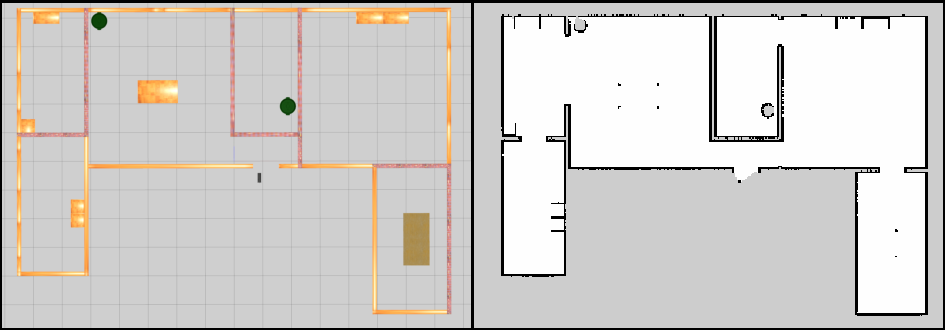
\includegraphics[width=\linewidth]{tb3-house-ogm.pdf}
    \caption{Top-down view of the TurtleBot3 House in Gazebo, and its OGM representation (mind the open doors in the building).
        Grey pixels represent unknown area, black pixels are occupied, white pixels are free cells.
        1 pixel (cell) in the OGM has a size of $0.05 \times 0.05$ m. }
    \label{fig:tb3-house-ogm}
\end{figure}
\subsection{The Motion Model}\label{subsec:mot-model}
Now that the hardware and the underlying localization task is introduced, the two main parts of the
Bayesian recursion is going to be described in the following subsections: the motion model, and the measurement model.

The motion model is used to describe the probability distribution of
$p(\mathbf{x}_t | \mathbf{x}_{t-1},\mathbf{u}_t)$ in \eqref{eq:bayes-predict}. \linebreak
Without any external information, the pose of the robot at time $t$ can be estimated based on the previous pose
at time $t-1$, and the control input at time $t$. Naturally, this estimation will be corrupted by tire slippage and drift.
Due to the incremental nature, these errors are integrated over time, thus making the estimation more and more
uncertain.

The motion model describes this transition using the kinematic model of the agent.
Based on the inputs, two distinct probabilistic models can be established, introduced in \cite{Thrun2005}: the velocity motion model,
and the odometry motion model.
The latter is usually more accurate (stated in \cite{Thrun2005}),
furthermore, does not require a timestep explicitly as a parameter.
These beneficial properties make it the ideal choice for this localization task,
thus it is detailed in the following.

If the odometry of the robot is available (i.e. by integrating wheel encoder measurements),
they can be treated as a control input:
\begin{equation}\label{eq:odom-raw-input}
    \hat{\mathbf{u}}_t = (\overline{\mathbf{x}}_t\;\;\overline{\mathbf{x}}_{t-1})^\top =
    \left(\overline{x}_t\;\;\overline{y}_t\;\;\overline{\theta}_t\;\;\overline{x}_{t-1}\;\;\overline{y}_{t-1}\;\;\overline{\theta}_{t-1}\right)^\top.
\end{equation}
The key is the fact that the relative difference between
two consecutive odometry data is a good estimation of the relative difference between
the two consecutive true poses, if the timestep is sufficiently small.

The transition between the state $\mathbf{x}_{t-1}$ and $\mathbf{x}_{t}$ is simplified to a sequence of a rotation, a translation,
and another rotation.
These are indicated in Figure~\ref{fig:odom-mot-model}. with $\delta_{\mathrm{rot1}}$, $\delta_{\mathrm{trans}}$,
and $\delta_{\mathrm{rot2}}$ respectively.
It is important to mention that this separation to rotational and translational components is arbitrary
(introduced by Thrun et al. in~\cite{Thrun2005}); for another approach, see~\cite{Eliazar2004}.
\begin{figure}[htbp]
    \centering
    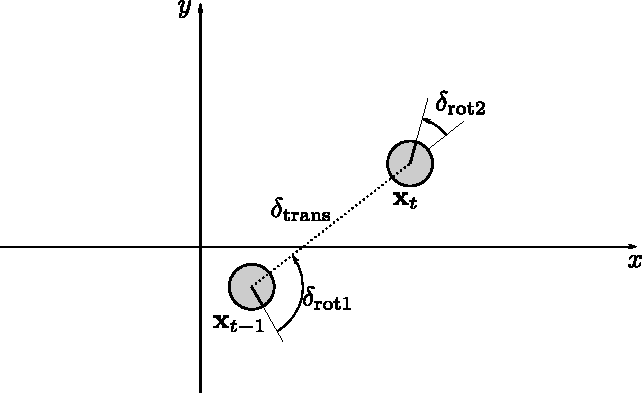
\includegraphics{odometry-motmodel.pdf}
    \caption{Rotation-translation-rotation transition sequence from state $\mathbf{x}_{t-1}$ to $\mathbf{x}_{t}$.}
    \label{fig:odom-mot-model}
\end{figure}

The odometry control input $\hat{\mathbf{u}}_t$
then transformed to the three transition components as:
\begin{align}
    \delta_{\mathrm{rot1,t}} & =\arctan\!2\left(\overline{y}_{t}-\overline{y}_{t-1}, \overline{x}_{t}-\overline{x}_{t-1}\right)-\overline{\theta}_{t-1}, \\
    \delta_{\text {trans,t}} & =\sqrt{\left(\overline{x}_{t-1}-\overline{x}_{t}\right)^{2}+\left(\overline{y}_{t-1}-\overline{y}_{t}\right)^{2}},        \\
    \delta_{\mathrm{rot2,t}} & =\overline{\theta}_{t}-\overline{\theta}_{t-1}-\delta_{\mathrm{rot} 1},                                                   \\
    \mathbf{u}_t             & = (\delta_{\text{rot1,t}}\;\;\delta_{\text{trans,t}}\;\;\delta_{\text{rot2,t}})^{\top}. \label{eq:odom-delta-input}
\end{align}
To model odometry noise, the inputs are treated as random variables, formulated by
\begin{align}
    \hat{\delta}_{\mathrm{rot1,t}} & = \delta_{\mathrm{rot1,t}} + \xi_{\mathrm{rot1,t}},
    \quad                          & \xi_{\mathrm{rot1,t}} \sim \mathcal{N}(0,\alpha_1\delta_{\mathrm{rot1,t}}^2+\alpha_2\delta_{\mathrm{trans,t}}^2), \label{eq:odom-control-1}                               \\
    \hat{\delta}_{\text {trans,t}} & = \delta_{\mathrm{trans,t}} + \xi_{\mathrm{trans,t}},
    \quad                          & \xi_{\mathrm{trans,t}} \sim \mathcal{N}(0,\alpha_3\delta_{\mathrm{trans,t}}^2+\alpha_4(\delta_{\mathrm{rot1,t}}^2+\delta_{\mathrm{rot2,t}}^2)), \label{eq:odom-control-2} \\
    \hat{\delta}_{\mathrm{rot2,t}} & = \delta_{\mathrm{rot2,t}} + \xi_{\mathrm{rot2,t}},
    \quad                          & \xi_{\mathrm{rot2,t}} \sim \mathcal{N}(0,\alpha_1\delta_{\mathrm{rot2,t}}^2+\alpha_2\delta_{\mathrm{trans,t}}^2), \label{eq:odom-control-3}
\end{align}
where $\alpha_1,\alpha_2,\alpha_3,\alpha_4$ are error parameters.

Then, using the control inputs and the previous state, samples from $p(\mathbf{x}_t | \mathbf{x}_{t-1},\mathbf{u}_t)$
are obtained by
\begin{align}
    x_t      & = x_{t-1} + \hat{\delta}_{\mathrm{trans,t}}\cos(\theta_{t-1} + \hat{\delta}_{\mathrm{rot1,t}}), \label{eq:prop-x} \\
    y_t      & = y_{t-1} + \hat{\delta}_{\mathrm{trans,t}}\sin(\theta_{t-1} + \hat{\delta}_{\mathrm{rot1,t}}), \label{eq:prop-y} \\
    \theta_t & = \theta_{t-1} + \hat{\delta}_{\mathrm{rot1,t}} + \hat{\delta}_{\mathrm{rot2,t}}. \label{eq:prop-theta}
\end{align}
This can be written in the form
\begin{equation}
    \mathbf{x}_t = \phi(\mathbf{x}_{t-1},\mathbf{u}_t,\mathbf{v}_t),
\end{equation}
where
\begin{align}
    \mathbf{x}_t & = (x_t\;\;y_t\;\;\theta_t)^{\top},                                            \\
    \mathbf{v}_t & = (\xi_{\text{rot1,t}}\;\;\xi_{\text{tans,t}}\;\;\xi_{\text{rot2,t}})^{\top}.
\end{align}
Based on \eqref{eq:odom-control-1}-\eqref{eq:odom-control-3}, the covariance matrix of the noise
vector $\mathbf{v}_t$ is
\begin{align}\label{eq:control-covar}
    \mathbf{Q}_t. := & \text{cov}(\mathbf{v}_t,\mathbf{v}_t) \nonumber \\
    =                &
    \text{diag}(\alpha_1\delta_{\mathrm{rot1,t}}^2+\alpha_2\delta_{\mathrm{trans,t}}^2,
    \alpha_3\delta_{\mathrm{trans,t}}^2+\alpha_4(\delta_{\mathrm{rot1,t}}^2+\delta_{\mathrm{rot2,t}}^2),
    \alpha_1\delta_{\mathrm{rot2,t}}^2+\alpha_2\delta_{\mathrm{trans,t}}^2).
\end{align}
For further usages, the Jacobians of $\phi$ are calculated:
\begin{align}
    \nabla\phi_x(\mathbf{x}_{t-1},\mathbf{u}_t) :=
    \left.\frac{\partial\phi}{\partial \mathbf{x}_{t-1}}\right\vert_{\mathbf{x}_{t-1},\mathbf{u}_t}
    =
     & \begin{bmatrix}
        1 & 0 & -\delta_{\text{trans,t}}\sin(\theta_{t-1} + \delta_{\text{rot1,t}}) \\
        0 & 1 & \delta_{\text{trans,t}}\cos(\theta_{t-1} + \delta_{\text{rot1,t}})  \\
        0 & 0 & 0
    \end{bmatrix}, \label{eq:motmodel-jacobi-x} \\
    \nabla\phi_u(\mathbf{x}_{t-1},\mathbf{u}_t) :=
    \left.\frac{\partial\phi}{\partial \mathbf{u}_{t}}\right\vert_{\mathbf{x}_{t-1},\mathbf{u}_t}
    =
     & \begin{bmatrix}
        -\delta_{\text{trans,t}}\sin(\theta_{t-1} + \delta_{\text{rot1,t}}) & \cos(\theta_{t-1} + \delta_{\text{rot1,t}}) & 0 \\
        \delta_{\text{trans,t}}\cos(\theta_{t-1} + \delta_{\text{rot1,t}})  & \sin(\theta_{t-1} + \delta_{\text{rot1,t}}) & 0 \\
        1                                                                   & 0                                           & 1
    \end{bmatrix}. \label{eq:motmodel-jacobi-u}
\end{align}

\pagebreak
\section{The Measurement Model}
\subsection{Introduction}
As the form of the motion model depends on many factors, for example the kinematics of the robot
(differential drive, car like structure, etc.), and the used control input interpretation
(odometry-based, or velocity-based), measurement models are no different.
However, the used exteroceptive sensor (LiDAR), and the utilized map representation (OGM)
for the localization task in scope narrows the possibilities.

This section details different measurement model realizations.
First, the basic principles are introduced for topological (feature based) maps,
then the beam range finder model for an OGM is further detailed.
However, these are not suitable for localization on an OGM with LiDAR measurements,
using a Kalman filter-based state estimation algorithm.
This is either due to the lack of a closed-form measurement equation (beam range finder model),
or the inability to process direct angle-range measurements.
As a solution, a Distance Function based measurement model  (\cite{Dantanarayana2013})
is applied. This model is described in the second half of the section.

\subsection{Standard Measurement Models on Different Map Realizations}
Wide-spread algorithms are often established for topological (feature-based) maps.
Here, the environment is described by detected shapes (features), rather than using a location based representation
like the OGMs do, as they assign an occupancy value for every location on the map.

For a topological map, the probability distribution of $p(\mathbf{\mathbf{z}}_t | \mathbf{x}_t)$,
enhanced with the known map $\mathbf{m}$ (resulting in $p(\mathbf{\mathbf{z}}_t | \mathbf{x}_t,\mathbf{m})$)
is described by a Gaussian distribution:
\begin{align}
    \psi(\mathbf{x}_t,\mathbf{m}) = \mathbf{z}^*_t + \xi, \quad \xi \sim \mathcal{N}(0,\mathbf{R}), \\
    \Rightarrow p(\mathbf{\mathbf{z}}_t | \mathbf{x}_t,\mathbf{m}) \sim \mathcal{N}(\mathbf{z}_t^*,\mathbf{R}),
\end{align}
where $\mathbf{R}$ is the covariance matrix of the measurement.
This closed-form description is required for Kalman Filters.

However, for location based (metric) maps, the form of $\mathbf{m}$ is different, therefore
to make the above model work, features have to be extracted \cite{Durrant-Whyte1991},
effectively making the map feature-based.

For purely metric maps (without feature extraction), Thrun et al. proposed the \emph{beam range finder model}
in \cite{Thrun2005}, especially fitted for range finders, like LiDARs, or sonars.
This model describes  $p(\mathbf{\mathbf{z}}_t | \mathbf{x}_t,\mathbf{m})$ as a composition of
probability densities, resulting in a distribution indicated in Figure \ref{fig:beam-model}.
Here, the value $\mathbf{z}_t^*$ is obtained by ray tracing: at a given robot pose,
the expected measurement can be calculated by tracing a ray along the map, starting form
the position of the robot, and ending with the nearest obstacle. Then the travelled distance is recorded,
which together with the angle of the beam, serves as $\mathbf{z}_t^*$.

The resulting distribution combines different measurement error possibilities:
random measurements (uniform distribution), local measurement noise (Gaussian distr.),
failures (``narrow'' uniform distribution, modelled by a Dirac delta) and unexpected
objects (exponential distribution).
\begin{figure}[htbp]
    \centering
    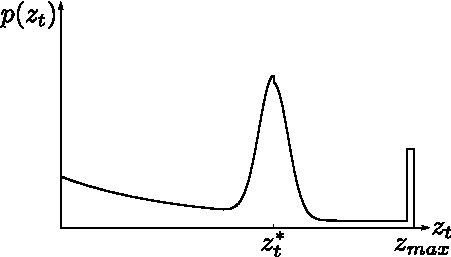
\includegraphics{beam-model.pdf}
    \caption{Probability distribution of $p(z_t | \mathbf{x}_t,\mathbf{m})$.
        The figure is based on \cite{Thrun2005}.}
    \label{fig:beam-model}
\end{figure}

However, the resulting probability distribution does not have a closed form description, which is
not a problem for particle filters, but it is for Kalman filters.

\subsection{The Distance Function based Measurement Model}\label{subsec:dt-meas-model}
The method, which enables the use of Kalman filters with laser range finder measurements on an OGM is proposed
by Dantanarayana et al. in \cite{Dantanarayana2013,Dantanarayana2016}.
In the following, this method is going to be detailed, based on \cite{Dantanarayana2016b}.

The key idea is the utilization of the distance transform (DT) operator, which is widely used in
image processing.
For a given binary image (or in this case, an OGM), the distance transform
produces an image/map (with the same size), where the value of each pixel/cell is
determined by the closest distance to any occupied pixel/cell,
by the evaluation of the distance function (DF).
If $V$ is the set of the occupied cells, and $\mathbf{x}$ is the position of an arbitrary cell on the map, then
\begin{equation}
    d_{D F}=D F(\mathbf{x})=\min _{\mathbf{v}_{\mathbf{j}} \in V}\left\|\mathbf{x}-\mathbf{v}_{\mathbf{j}}\right\|,
\end{equation}
in which an Euclidean norm is usually applied.
The distance transform then could be pre-calculated for a given map.
Figure \ref{fig:simple-dt}. shows the DT in a simplified environment,
while the DT of the OGM from Figure \ref{fig:tb3-house-ogm}. can be seen on Figure \ref{fig:gazebo-map-ogm-dt}.
\begin{figure}[htbp]
    \centering
    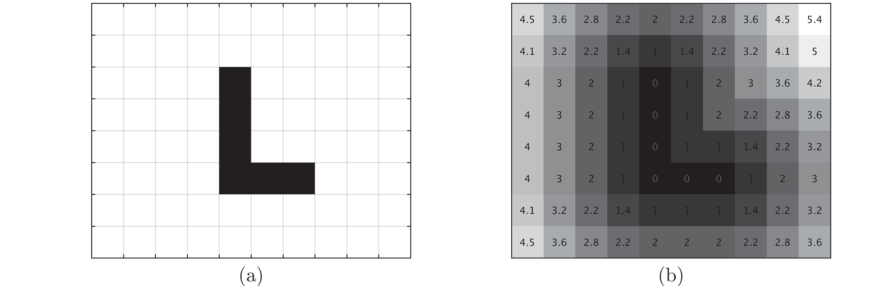
\includegraphics{simple_dt.pdf}
    \caption{A simple shape and its distance transform. Figure source: \cite{Dantanarayana2016b}.}
    \label{fig:simple-dt}
\end{figure}
\begin{figure}[htbp]
    \centering
    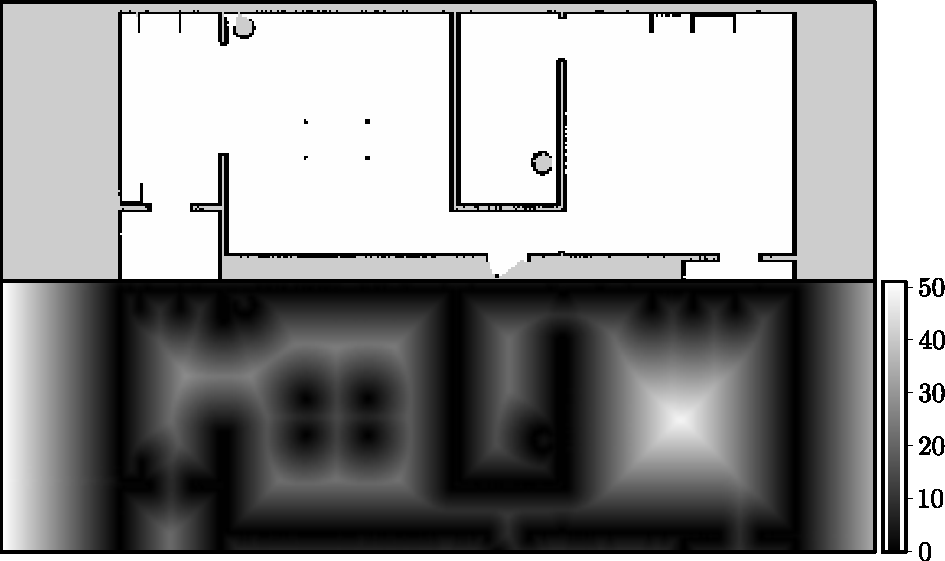
\includegraphics{dt_on_ogm.pdf}
    \caption{Part of the OGM of the TurtleBot3 House, and its distance transform.}
    \label{fig:gazebo-map-ogm-dt}
\end{figure}

Now using the LiDAR measurements, which in this case come in the form of angle-range pairs,
each detection can be transformed to map coordinates, and assigned a distance function value.
Theoretically, if the estimated pose of the robot, and the true pose of the robot aligns,
and the sensor is noiseless, each reading should indicate an occupied cell on the OGM.
Therefore, all the projected detections should have a DT of 0.
In other cases, the ray endpoints could end up on free cells, thus having a DT value larger,
than 0.

The method of transforming (projecting) the laser scans to the map, based on the estimated
location of the robot is shown in Figure \ref{fig:ogm-laser-projection}.
Mathematically, these projections are obtained as
\begin{equation}\label{eq:ray-projection}
    \mathbf{x}_{\mathrm{o}i} = \begin{bmatrix}x_{\mathrm{o}i}\\y_{\mathrm{o}i}\end{bmatrix}
    = \begin{bmatrix}x + r_i\cos(\varphi_i + \theta)\\y + r_i\sin(\varphi_i + \theta)\end{bmatrix},
\end{equation}
where the variables are according to Figure \ref{fig:ogm-laser-projection}. (the time dependency is omitted).
\begin{figure}[htbp]
    \centering
    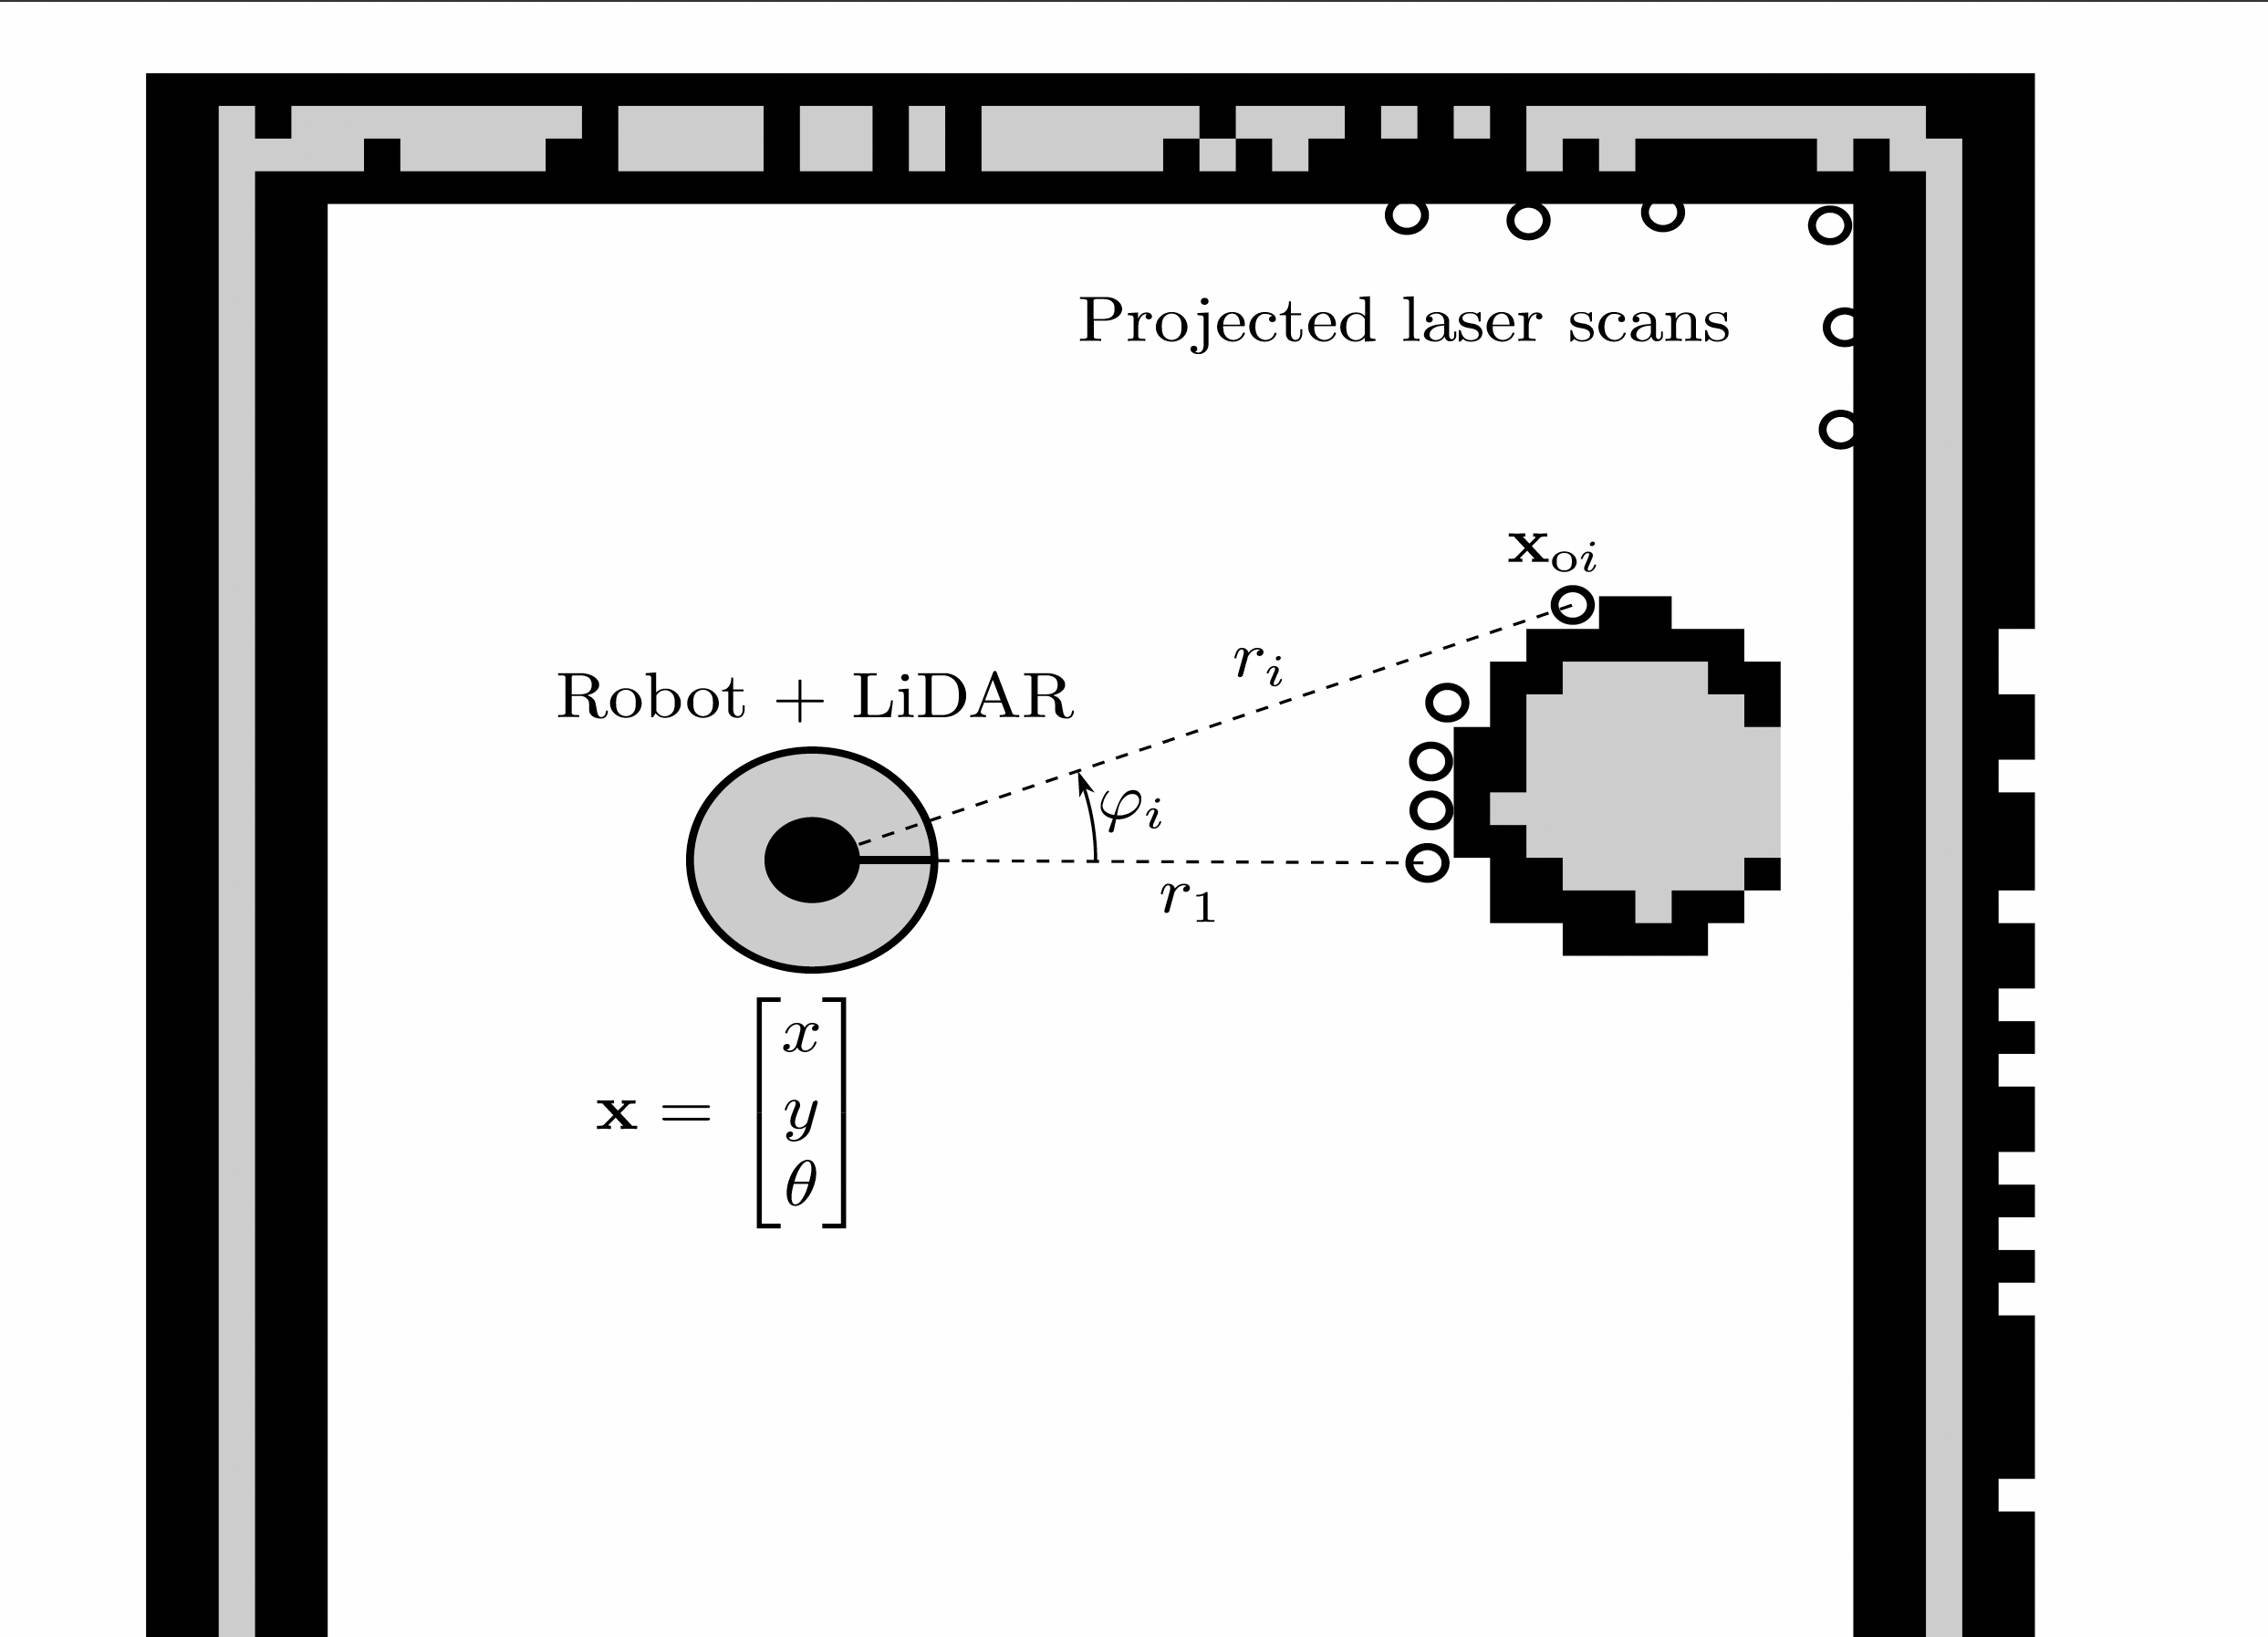
\includegraphics[width=0.8\linewidth]{dt_mapping_lidar}
    \caption{Projection of the LiDAR scans to the OGM, based on the pose of the robot.
    The rotating LiDAR emits a certain number of laser rays,
    here pictured by dashed lines for the first ray and the $i$-th ray
    (others are omitted for the sake of readability).
    The received measurement for the $i$-th ray is the length of the ray $r_i$,
    and the ray angle $\varphi_i$, measured relative from the heading of the robot,
    indicated by a thick black line.
    The ray endpoint then projected onto the map, resulting $\mathbf{x}_{\text{o}i}$ for the $i$-th ray.}
    \label{fig:ogm-laser-projection}
\end{figure}

Based on a set of measurements (for a whole revolution of the LiDAR), a vector can be constructed as follows:
\begin{equation}\label{eq:df-vector}
    \mathbf{d}_{\text{DF}} =
    \begin{bmatrix}
        DF(\mathbf{x}_{\text{o}1}) \\
        DF(\mathbf{x}_{\text{o}2}) \\
        \vdots                     \\
        DF(\mathbf{x}_{\text{o}n}) \\
    \end{bmatrix},
\end{equation}
where $n$ is the number of valid LiDAR readings for a whole revolution
(a valid reading occurs when the laser ray actually collided with an object within range, and this was
detected by the sensor).

By mapping the ray endpoints to the map, the resulting point lies
on a continuous space.
However, the distance transform of the OGM is obtained by
the distance function, which is only defined for discrete positions
on the map (the cell midpoints), not for continuous coordinates.
Instead of the quantization of the ray endpoint coordinates, a cubic spline
interpolation is applied on the distance field,
enabling the evaluation of the DF for continuous coordinates as well.
This approach also eliminates the problem of calculating the
partial derivative of the DF with respect to $x$ or $y$,
which is not defined at $x = \hat{x}, y = \hat{y}$, where
$(\hat{x}\;\; \hat{y})^{\top}$ is the coordinates of an occupied cell.
Instead, use the corresponding partial derivatives of the interpolated spline.


To obtain a single scalar value, which indicates the disparity between the projected measurements,
and the map, the Chamfer Distance (CD) is formulated. For a set of measurements,
\begin{equation}
    d_{\text{CD}} = \frac{1}{n}\sum_{i=1}^nDF(\mathbf{x}_{\text{o}i}).
\end{equation}
The CD is a good indicator for the estimation of the robot's pose: $\mathrm{CD}=0$ means
that every ray endpoint for a set of measurement at time $t$ is at the right place,
therefore the initial robot pose estimation is good.
Although, it is important to mention that this assumption does not hold in every
scenario. Consider an extreme case: for a whole revolution, the LiDAR only records
one measurement (one ray), and the OGM contains many occupied cells.
Then the CD (effectively the DT) would equal to zero at a plethora of robot poses, thus not indicating the sought true pose.
For a detailed map and sufficiently many LiDAR readings per revolution, this deficiency is minimized.

Using the CD, the measurement model is formulated as
\begin{equation}
    p(\mathbf{\mathbf{z}}_t | \mathbf{x}_t, DF_t) \sim \mathcal{F}(d_{\text{CD}t},\boldsymbol\Sigma_{\text{CDt}}),
\end{equation}
where $\mathcal{F}$ denotes the folded Gaussian distribution (this comes from the fact that the codomain of the DF is nonnegative).
The covariance is calculated as
\begin{equation}\label{eq:cd-covariance}
    \boldsymbol\Sigma_{\text{CD}} = \mathbf{J}_{\text{CD}}\mathbf{R}\mathbf{J}_{\text{CD}}^{\top},
\end{equation}
where $\mathbf{R}$ is the measurement covariance matrix, and $\mathbf{J}_{CD}$ is the Jacobian of the
Chamfer distance with respect to $\mathbf{z}_i = (\varphi_i\;\;r_i)$,
evaluated at $\mathbf{x}$.
For a LiDAR, the uncertainty of the angle measurements $\varphi_i$ is often not considered,
therefore $\mathbf{R}$ can be formulated as,
\begin{equation}\label{eq:lidar-meas-covar}
    \mathbf{R} = \sigma_r^{2}\mathbf{I}_{n\times n},
\end{equation}
where $\sigma_r$ is the standard derivation of $r_i$ (same for every ray),
and $\mathbf{I}_{n\times n}$ is the identity matrix with size $n\times n$,
if $n$ is the number of valid readings for a whole revolution of the LiDAR.
Using this simplification, the Jacobian in \eqref{eq:cd-covariance}
is only calculated with respect to $r_i$.

The observation function $\psi$ is defined as:
\begin{equation}\label{eq:observation-function}
    \psi(\mathbf{x},\mathbf{z}) = d_{\text{CD}} = \frac{1}{n}\sum_{i=1}^{n}DF(\mathbf{x}_{\text{o}i}).
\end{equation}
If the measurement $\mathbf{z}$ is not corrupted by noise, and the state $\mathbf{x}$
is at the true state (where the measurement was actually recorded), the observation
function has the value of
\begin{equation}\label{eq:impl-meas-eq}
    \psi(\mathbf{x},\mathbf{z}) = 0,
\end{equation}
forming an implicit measurement equation.


For further usages, the Jacobians of $\psi$ have to be formulated.
The Jacobian with respect to $\mathbf{x}$ is
\begin{equation}\label{eq:measmodel-jacobi-x}
    \nabla\psi_x(\mathbf{x},\mathbf{z}) := \left.\frac{\partial\psi}{\partial \mathbf{x}}\right\vert_{\mathbf{x},\mathbf{z}} =
    \frac{1}{n}
    \begin{bmatrix}
        \cfrac{1}{n}\displaystyle\sum\limits_{i=1}^{n}\left(\cfrac{\partial DF(\mathbf{x}_{\text{o}i})}{\partial x_{\text{o}}}\cfrac{\partial x_{\text{o}}}{\partial x}\right) \\
        \cfrac{1}{n}\displaystyle\sum\limits_{i=1}^{n}\left(\cfrac{\partial DF(\mathbf{x}_{\text{o}i})}{\partial y_{\text{o}}}\cfrac{\partial y_{\text{o}}}{\partial y}\right) \\
        \cfrac{1}{n}\displaystyle\sum\limits_{i=1}^{n}\left(\cfrac{\partial DF(\mathbf{x}_{\text{o}i})}{\partial x_{\text{o}}}\cfrac{\partial x_{\text{o}}(\mathbf{x},\mathbf{z}_i)}{\partial \theta}
        + \cfrac{\partial DF(\mathbf{x}_{\text{o}i})}{\partial y_{\text{o}}}\cfrac{\partial y_{\text{o}}(\mathbf{x},\mathbf{z}_i)}{\partial \theta}\right)                     \\
    \end{bmatrix}^{\top}.
\end{equation}
Here, the partial derivatives of the DF are obtained via the interpolated spline, therefore the analytical
derivation is not required.
The partial derivatives of $x_o$ and $y_o$ are trivial according to \eqref{eq:ray-projection}.

The Jacobian with respect to $\mathbf{z} = (\mathbf{z}_1\;\;\mathbf{z}_2\;\; \dots \;\; \mathbf{z}_n)^{\top}$ is simplified due to the fact that the noise effecting the
angle measurements $\varphi_i$ is neglected, therefore only the partial derivatives with respect to $r_i$ have to
be calculated:
\begin{align}\label{eq:measmodel-jacobi-z}
    \nabla\psi_z(\mathbf{x},\mathbf{z}) := \left.\frac{\partial\psi}{\partial \mathbf{z}}\right\vert_{\mathbf{x},\mathbf{z}}
     & =
    \frac{1}{n}
    \begin{bmatrix}
        \cfrac{\partial DF(\mathbf{x}_{\text{o}1})}{\partial x_{\text{o}}}\cfrac{\partial x_{\text{o}}(\mathbf{x},\mathbf{z}_1)}{\partial r_1}
        + \cfrac{\partial DF(\mathbf{x}_{\text{o}1})}{\partial y_{\text{o}}}\cfrac{\partial y_{\text{o}}(\mathbf{x},\mathbf{z}_1)}{\partial r_1} \\
        \cfrac{\partial DF(\mathbf{x}_{\text{o}2})}{\partial x_{\text{o}}}\cfrac{\partial x_{\text{o}}(\mathbf{x},\mathbf{z}_2)}{\partial r_2}
        + \cfrac{\partial DF(\mathbf{x}_{\text{o}2})}{\partial y_{\text{o}}}\cfrac{\partial y_{\text{o}}(\mathbf{x},\mathbf{z}_2)}{\partial r_2} \\
        \vdots                                                                                                                                   \\
        \cfrac{\partial DF(\mathbf{x}_{\text{o}n})}{\partial x_{\text{o}}}\cfrac{\partial x_{\text{o}}(\mathbf{x},\mathbf{z}_n)}{\partial r_n}
        + \cfrac{\partial DF(\mathbf{x}_{\text{o}n})}{\partial y_{\text{o}}}\cfrac{\partial y_{\text{o}}(\mathbf{x},\mathbf{z}_n)}{\partial r_n} \\
    \end{bmatrix}^{\top}.
\end{align}
\pagebreak
\section{State Estimators for Localization}\label{sec:state-estimators}
\subsection{Introduction}

In the previous sections, all of the preliminary components for
state estimation were discussed:
the Bayes filter as a foundation;
the motion and the measurement models based on the
sensors and the kinematics of the actual robot;
and the representation of the environment as an OGM.

The main goal of this section is to introduce the Exact Flow Daum--Huang filter. However, to properly understand the motivation behind
the creation of the filter along with its strengths and weaknesses, first the
examination of the Kalman filters and the particle filters are necessary.

Besides that Kalman filters are essential to understand state estimation,
the extended Kalman Filter (EKF) is directly required for the implemented Daum--Huang filter variant. For this special localization task with
an implicit measurement equation, the implicit extension of the EKF is provided, based on the literature.

As Daum--Huang filters are mainly developed to specifically overcome
an important deficiency of particle filters, their detailing is
also required. This is done through the examination of the bootstrap particle filter algorithm.

Finally, the Daum--Huang filters are discussed in general,
followed by the Exact Flow Daum--Huang filter (EDH). Similarly to the EKF,
an implicit extension is also required here to suit the
specific localization task. Such method is  yet not to be found in the literature, therefore lies within the contributions
of this report. As a summary, the complete pseudocode for the implemented EDH algorithm is provided in the last subsection.
\subsection{The Kalman Filters}
\subsubsection{Kalman Filter}
The Kalman filter (KF) assumes that ``everything'' \emph{is} linear and Gaussian,
and under these assumptions it can be proved that ``everything'' \emph{stays} linear and Gaussian during the Bayes filter updates.
A Gaussian distribution can be fully characterized by its first two moments,
therefore the Kalman filter offers a recursion to calculate the mean $\boldsymbol{\mu}_t$ and the covariance $\mathbf{\Sigma}_t$ of the belief $bel(\mathbf{x}_t)$.
In this context only the discrete-time KF is going to be discussed.

Consider the discrete-time (linear) state space model of a controlled system:
\begin{align}
  \mathbf{x}_t & = \mathbf{A}_t\mathbf{x}_{t-1} + \mathbf{B}_t\mathbf{u}_t + \mathbf{B}_t\mathbf{v}_t, \\
  \mathbf{z}_t & = \mathbf{C}_t\mathbf{x}_t + \mathbf{w}_t, \label{eq:lin-meas-model}
\end{align}
% ! TODO v és w kicserél
where $\mathbf{A}_t$ is the state transition matrix, $\mathbf{B}_t$ is the input gain, and $\mathbf{C}_t$ is the measurement matrix. To incorporate uncertainties and inaccuracies into the system,
the control noise $\mathbf{v}_t$ and the measurement noise $\mathbf{w}_t$ is introduced.
Both are Gaussian random variables:
$\mathbf{v}_t \sim \mathcal{N}(\mathbf{0},\mathbf{Q})$, $\mathbf{w}_t \sim \mathcal{N}(\mathbf{0},\mathbf{R})$,
with $\mathbf{Q}$ as control noise covariance, and $\mathbf{R}$ as measurement noise covariance.

Using the linear nature of the model, and assuming, that the probability distributions in the Bayes filter are Gaussian distributions, the motion model has the following form:
\begin{equation}\label{key}
  p(\mathbf{x}_t|\mathbf{x}_{t-1}, \mathbf{u}_t) = \mathrm{det}(2\pi\tilde{\mathbf{Q}}_t)
  ^{-\frac{1}{2}}\mathrm{exp}\{-\frac{1}{2}(\mathbf{x}_t-\mathbf{A}_t\mathbf{x}_{t-1}-
  \mathbf{B}_t\mathbf{u}_t)^\top\tilde{\mathbf{Q}}_t^{-1}(\mathbf{x}_t-\mathbf{A}_t\mathbf{x}_{t-1}-\mathbf{B}_t\mathbf{u}_t)\},
\end{equation}
where $\tilde{\mathbf{Q}}_t = \mathbf{B}_t\mathbf{Q}_t\mathbf{B}_t^{\top}$.
The measurement model can be calculated similarly.

The derivation of the Kalman filter algorithm is not trivial, and does not fall within the scope of this document. The algorithm can be seen in Algorithm \ref{alg:kf}., where $\mathbf{I}$ denotes the identity matrix, $\mathbf{z}'_t$ is the actual measurement.

\begin{algorithm}
  \caption{Kalman filter($\boldsymbol{\mu}_{t-1},\mathbf{\Sigma}_{t-1},\mathbf{u}'_t,\mathbf{z}'_t$)}\label{alg:kf}
  \begin{algorithmic}[1]
    \BState \emph{prediction}:
    \State\indent$\overline{\boldsymbol{\mu}}_t = \mathbf{A}_t{\boldsymbol{\mu}}_{t-1} + \mathbf{B}_t\mathbf{u}'_t$
    \State\indent $\overline{\mathbf{\Sigma}}_t = \mathbf{A}_t\mathbf{\Sigma}_{t-1}\mathbf{A}^\top_t + \tilde{\mathbf{Q}}_t$
    \BState \emph{update/correction}:
    \State\indent $\mathbf{K}_t = \overline{\mathbf{\Sigma}}_t\mathbf{C}_t^\top\left(\mathbf{C}_t\overline{\mathbf{\Sigma}}_t\mathbf{C}_t^\top+\mathbf{R}_t\right)^{-1}$
    \State\indent $\boldsymbol{\mu}_t = \overline{\boldsymbol{\mu}}_t + \mathbf{K}_t\left(\mathbf{z}'_t-\mathbf{C}_t\overline{\boldsymbol{\mu}}_t\right)$
    \State\indent $\mathbf{\Sigma}_t = \left(\mathbf{I}-\mathbf{K}_t\mathbf{C}_t\right)\overline{\mathbf{\Sigma}}_t$
    \State\Return $\boldsymbol{\mu}_t,\mathbf{\Sigma}_t$
  \end{algorithmic}
\end{algorithm}
\subsubsection{Extended Kalman Filter}
However, assuming a linear state space model is a rather strong assumption. For a nonlinear model the general state space equations are:
\begin{align}
  \mathbf{x}_t & = \phi(\mathbf{x}_{t-1},\mathbf{u}_t,\mathbf{v}_t) \label{eq:explicit-mot-eq} \\
  \mathbf{z}_t & = \psi(\mathbf{x}_t,\mathbf{w}_t).  \label{eq:explicit-meas-eq}
\end{align}
The state propagation function $\phi$ can be locally linearized about $\mathbf{x}_{t-1} = \boldsymbol{\mu}_{t-1}, \mathbf{u}_t = \mathbf{u}'_t$ with respect to $\mathbf{x}_{t-1}$ and $\mathbf{u}_t$, resulting in $\nabla \phi _x(\boldsymbol{\mu}_{t-1},\mathbf{u}'_t)$ and $\nabla \phi_u(\boldsymbol{\mu}_{t-1},\mathbf{u}'_t)$.
The measurement function $\psi$ is linearized about the current predicted state $\overline{\boldsymbol{\mu}}_t$,
resulting in $\nabla \psi_x(\overline{\boldsymbol{\mu}}_t)$.
In Algorithm \ref{alg:ekf}., the arguments of these Jacobians are omitted.

As a summarization, the EKF algorithm (see in Algorithm \ref{alg:ekf}.) is the extension of the KF by handling nonlinear state equations through their Jacobians.

\begin{algorithm}
  \caption{Extended Kalman filter($\boldsymbol{\mu}_{t-1},\mathbf{\Sigma}_{t-1},\mathbf{u}'_t,\mathbf{z}'_t$)}\label{alg:ekf}
  \begin{algorithmic}[1]
    \BState \emph{prediction}:
    \State\indent$\overline{\boldsymbol{\mu}}_t = \phi(\boldsymbol{\mu}_{t-1},\mathbf{u}'_t,0)$
    \State\indent $\overline{\mathbf{\Sigma}}_t = \nabla \phi_x\mathbf{\Sigma}_{t-1}\nabla \phi_x^{\top} +
      \nabla \phi _u\mathbf{Q}_t \nabla \phi_u^{\top}$
    \BState \emph{update/correction}:
    \State\indent $\mathbf{K}_t = \overline{\mathbf{\Sigma}}_t\nabla \psi_x^\top\left(\nabla \psi_x\overline{\mathbf{\Sigma}}_t\nabla \psi_x^\top+\mathbf{R}_t\right)^{-1}$ \label{alg:line:kalman-gain}
    \State\indent $\boldsymbol{\mu}_t = \overline{\boldsymbol{\mu}}_t + \mathbf{K}_t\left(\mathbf{z}'_t-\psi(\overline{\boldsymbol{\mu}}_t,0)\right)$ \label{alg:line:state-update}
    \State\indent $\mathbf{\Sigma}_t = \left(\mathbf{I}-\mathbf{K}_t\nabla \psi_x\right)\overline{\mathbf{\Sigma}}_t$
    \State\Return $\boldsymbol{\mu}_t,\mathbf{\Sigma}_t$
  \end{algorithmic}
\end{algorithm}

\subsubsection{EKF for Implicit Measurement Equation}

The standard KF and EKF assume an explicit measurement equation in the form of \eqref{eq:explicit-meas-eq}.
However, as stated in Subsection \ref{subsec:dt-meas-model}, the measurement equation for the inspected
localization problem has an implicit form of \eqref{eq:impl-meas-eq}.
To suit this condition, Algorithm \ref{alg:ekf}. has to be modified, based on \cite{Steffen2013,Zhang2012}.
Line \ref{alg:line:kalman-gain}. is changed to
\begin{equation}
  \mathbf{K}_t = \overline{\mathbf{\Sigma}}_t\nabla \psi_x^\top\left(\nabla \psi_x\overline{\mathbf{\Sigma}}_t\nabla \psi_z^\top+
  \nabla \psi_z\mathbf{R}_t\nabla \psi^{\top}_z\right)^{-1},
\end{equation}
where $\nabla \psi_z$ is the Jacobian of $\psi$ with respect to $\mathbf{z}_t$, evaluated at
$\mathbf{x}_t = \overline{\boldsymbol{\mu}}_t, \mathbf{z}_t = \mathbf{z}'_t$.
Furthermore, because the expected output of the observation function is 0, Line \ref{alg:line:state-update}. in Algorithm~\ref{alg:ekf}. has the modified form
\begin{equation}
  \boldsymbol{\mu}_t = \overline{\boldsymbol{\mu}}_t + \mathbf{K}_t\left(0-\psi(\overline{\boldsymbol{\mu}}_t,\mathbf{z}'_t)\right).
\end{equation}
\subsubsection{Advantages and Disadvantages of Kalman Filters}

Under linear and Gaussian assumptions the Kalman filter yields the optimal estimation (by calculated mean squared error). However, these criteria are rarely satisfied, and the optimal estimation property does not hold any more. Another major problem comes from the nature of Gaussian distributions: they are unimodal, therefore the Kalman Filter cannot track multiple high-probability hypotheses.

EKF offers one type of solution to the nonlinearity: linearization by Taylor expansion. This however, introduces linearization error into the system. For highly nonlinear equations not only the first order approximation is the problem, but its center point as well. As were mentioned before, the state equation is linearized around the previous state; but now this state is also an approximation. This overall effect can cause the algorithm to diverge, or to yield poor results. In addition, the initial conditions also have to be carefully chosen in order to obtain desired results.

Despite these, the EKF is still one of the most popular state estimation algorithm in robotics, and often used in Global Navigation Satellite Systems (GNSS) as well, thanks to its computational simplicity and easy  implementation. Other Kalman filter based realizations are including but not limited to the unscented Kalman filter \cite{Julier2004}, which uses sigma points to track the evolution of the density, and the ensemble Kalman Filter \cite{Evensen2003}, which is suited for high dimensional estimation problems.

\subsection{The Particle Filters}
\subsubsection{Main concepts}

Particle filters (PF) are used to solve nonlinear filtering problems. Unlike EKF and other nonlinear extensions of the Kalman filter, this method uses a nonparametric representation of the estimated posterior. This nonparametric nature enables the estimation of various distributions, including multimodal and/or non-Gaussian.

The main concept in PF is to represent arbitrary probability distributions by cumulative probability mass of particles. When for example a Gaussian distribution is sampled multiple times, more samples come from regions with high probability density. This (trivial) effect can also be used in reverse: if samples are given, what is the probability distribution from which they were sampled? If the number of particles is sufficiently large (ideally infinity), they can offer a good approximation of the generating probability distribution.

The Bayesian filtering framework is implemented as follows. First, draw $N$ samples (called as particles) from a prior distribution. Then migrate each of these particles according to the motion model. Now the particle set will approximately describe the predicted belief \eqref{eq:predbel}. (In the KF this predicted belief was described by its mean and covariance, as it was assumed to be a Gaussian distribution. Now, it is described by particles, and the Gaussian nature is not required.)

The KF used the $\mathbf{K}_t$ Kalman gain as a weight to calculate the posterior from the predicted belief. Particle filters use \emph{importance sampling} for this task: each sample is given an importance weight which describes its relevance. If this relevance is high, it means that the specific particle is a good approximation of the true (sought) state. Choosing a proper weighting method is a difficult task. Generally, weights are calculated from a target and a proposal distribution. The target distribution is the posterior, the proposal distribution however, can be arbitrary (under some criteria). Now using the particles and their weights, the posterior distribution is approximated.

The next step of the filter is optional, although essential: resampling. Here, a new (same sized) particle set is constructed by drawing particles from the old set with replacement, according to their weights. This means that some  particles can be chosen multiple times (more likely high-weighted ones), thus certain particles can be eliminated. Finally, their weights are equalized. With the resulting particle set (either the new, redrawn one, or the old, weighted one), the algorithm is repeated in the new time step.

Generally, the most demanding task when designing PFs is the proper selection of the proposal density and the resampling frequency (i.e. when to resample). Choosing the right proposal distribution and the right time to resample is crucial in the performance of the PF. In the next subsection, the bootstrap particle filter method with adaptive resampling is introduced in detail.
\subsubsection{The Bootstrap Particle Filter}

Denote the particles and their set at time $t$  as:
\begin{equation}\label{key}
  \mathcal{X}_t = \{\mathbf{x}_t^{[1]},\mathbf{x}_t^{[2]}, \dots \mathbf{x}_t^{[N]}\}.
\end{equation}

The bootstrap particle filter uses the predicted belief as the proposal distribution, which results in the following weight assignment:
\begin{equation}\label{key}
  w_t^{[n]} = p(\mathbf{z}_t|\mathbf{x}_t^{[n]}).
\end{equation}
This means, that  if the proposal distribution is the predicted belief, the weight is calculated according to the measurement model (the mathematical derivation is omitted). In the original algorithm \cite{Gordon1993}, resampling is performed in every step. However, this might not be beneficial, therefore an effective sample size based adaptive resampling is applied \cite{Liu2004}. One major problem with particle filters is when many particles are in irrelevant locations, therefore only a few of them represent the high probability region of the posterior properly. This phenomenon is called particle degeneracy. However, the value of the weights can indicate this ill-favored situation. The effective sample size ($ESS$ or $N_{\mathrm{eff}}$) can be approximated as the following:
\begin{equation}\label{eq:neff}
  N_{\mathrm{eff}} = \frac{1}{\sum_{i = 1}^{N}(w_t^{[i]})^2},
\end{equation}
if the sum of weights are 1 (normalized). Consider the situation where all the weights are equal, thus $w_t^{[1]} = w_t^{[2]} = \dots = w_t^{[N]} = 1/N$. This results in $N_{\mathrm{eff}} = N$, which is beneficial. The worst case scenario is when one weight is 1, and all the others are 0, which results in $N_{\mathrm{eff}} = 1$. It is common to define a threshold $N_{T}$, where if $N_{\mathrm{eff}} < N_T$, a resampling is performed.

The pseudocode of the bootstrap particle filter with adaptive resampling is presented in Algorithm \ref{alg:bpf}.
\begin{algorithm}[b!]
  \caption{Bootstrap particle filter ($\mathcal{X}_{t-1}, \mathbf{u}_t, \mathbf{z}'_t$)}\label{alg:bpf}
  \begin{algorithmic}[1]
    \State $\overline{\mathcal{X}}_t = \mathcal{X}_t = \emptyset$
    \For{ $n$ = 1 to $N$ }
    \State sample $\mathbf{x}_t^{[n]} \sim p(\mathbf{x}_t|\mathbf{x}_{t-1}^{[n]},\mathbf{u}_t)$
    \State$w_t^{[n]} = p(\mathbf{z}_t = \mathbf{z}'_t|\mathbf{x}_{t}^{[n]})w_{t-1}^{[n]}$
    % ! Gausst
    \EndFor
    \State calculate weight sum $\hat{w}_{t} = \sum_{i = 1}^{N}w_t^{[i]}$
    \For{ $n$ = 1 to $N$ }
    \State normalize $w_t^{[n]} = w_t^{[n]}\hat{w}_t^{-1}$
    \State$\overline{\mathcal{X}}_t = \overline{\mathcal{X}}_t + \langle \mathbf{x}_t^{[n]},w_t^{[n]}\rangle$
    \EndFor
    \State calculate $N_{\mathrm{eff}}$ using \eqref{eq:neff}
    \If{$N_{\mathrm{eff}} < N_T$}
    \For{ $n$ = 1 to $N$ }
    \State draw $i$ with probability $\propto w_t^{[i]}$ \label{line:bpf_resaml}
    \State${\mathcal{X}}_t ={\mathcal{X}}_t + \langle \mathbf{x}_t^{[i]},N^{-1}\rangle$
    \EndFor
    \State\Return $\mathcal{X}_t$
    \Else
    \State$\mathcal{X}_t = \overline{\mathcal{X}}_t$
    \State\Return $\mathcal{X}_t$
    \EndIf
  \end{algorithmic}
\end{algorithm}
There are several ways to implement the resampling in Line \ref{line:bpf_resaml}: the most basic method is the ''roulette wheel'' sampling, but in this scenario, the stratified sampling \cite{Li2015} is used.

\subsubsection{Adaptive Monte Carlo Localization}

For localization, one particularly popular method is the Adaptive Monte Carlo Localization (AMCL),
proposed in \cite{Fox2002}. It is also implemented in the ROS \cite{AMCLROS2002}, and serves as the de facto standard localization algorithm in the ROS community.
The basic concepts come from Monte Carlo Localization by particle filters,
detailed detailed  previously.
The main addition is the introduction of adaptive sample size, based on a
the Kullback-Leibler distance (KLD), which is a measure for approximation error.
If the uncertainty of the pose of the robot is high, the particle number
is increased in the next resampling process. If the pose approximation
is good, the particle set size is decreased for increased efficiency.

\subsubsection{Advantages and Disadvantages of Particle Filters}\label{sec:pf_adv_disadv}
Particle filters are well suited for nonlinear and non-Gaussian state estimation. They are especially versatile: many PF variations can be constructed for a plethora of applications. They are easy to implement, and demand low computational power (per particle).

However, its numeric solution method (approximate probability distributions by samples) leaves a lot of room for errors. Most importantly, the particle filter can suffer from the so called \emph{curse of dimensionality}, which is described in \cite{Gordon1993} as ``One must expect $N$ (the number of particles) to rise rapidly with the dimension of the space (...) It is most difficult to make any precise provable statement on the crucial question of how many samples are required to give a satisfactory representation of the densities for filter operation''. With a good proposal distribution, this unwanted property can be avoided. Daum and Huang showed in \cite{Daum2003}, that the BPF suffers from this phenomenon, while for example the unscented particle filter does not.

The curse of dimensionality problem is connected to particle degeneracy. It means that only a low amount of samples estimates the target posterior efficiently; others are in regions with very low probability. This occurs when the proposal distribution and the target distribution are not matched well. Figure \ref{fig:pf-degen}. shows a setup which demonstrates this effect: the prior distribution (the predicted belief in the case of the BPF) is colored in blue, and represented by its particles, shown as black dots. The weighting of the particles is done according to the likelihood (red curve), which is the measurement model in the BPF. As a result, only 3 particles are going to have weights other, than 0. Upon resampling, only these 3 particles will represent the target posterior; the others are eliminated. (Of course the size of the particle set will not change, only that they are distributed across 3 distinct positions). By common sense, a probability distribution is hardly represented properly by 3 particles. Counter-intuitively, having a more precise sensor (i.e. having a ''thinner'' likelihood function) only makes this worse.

\begin{figure}[htb!]
  \centering
  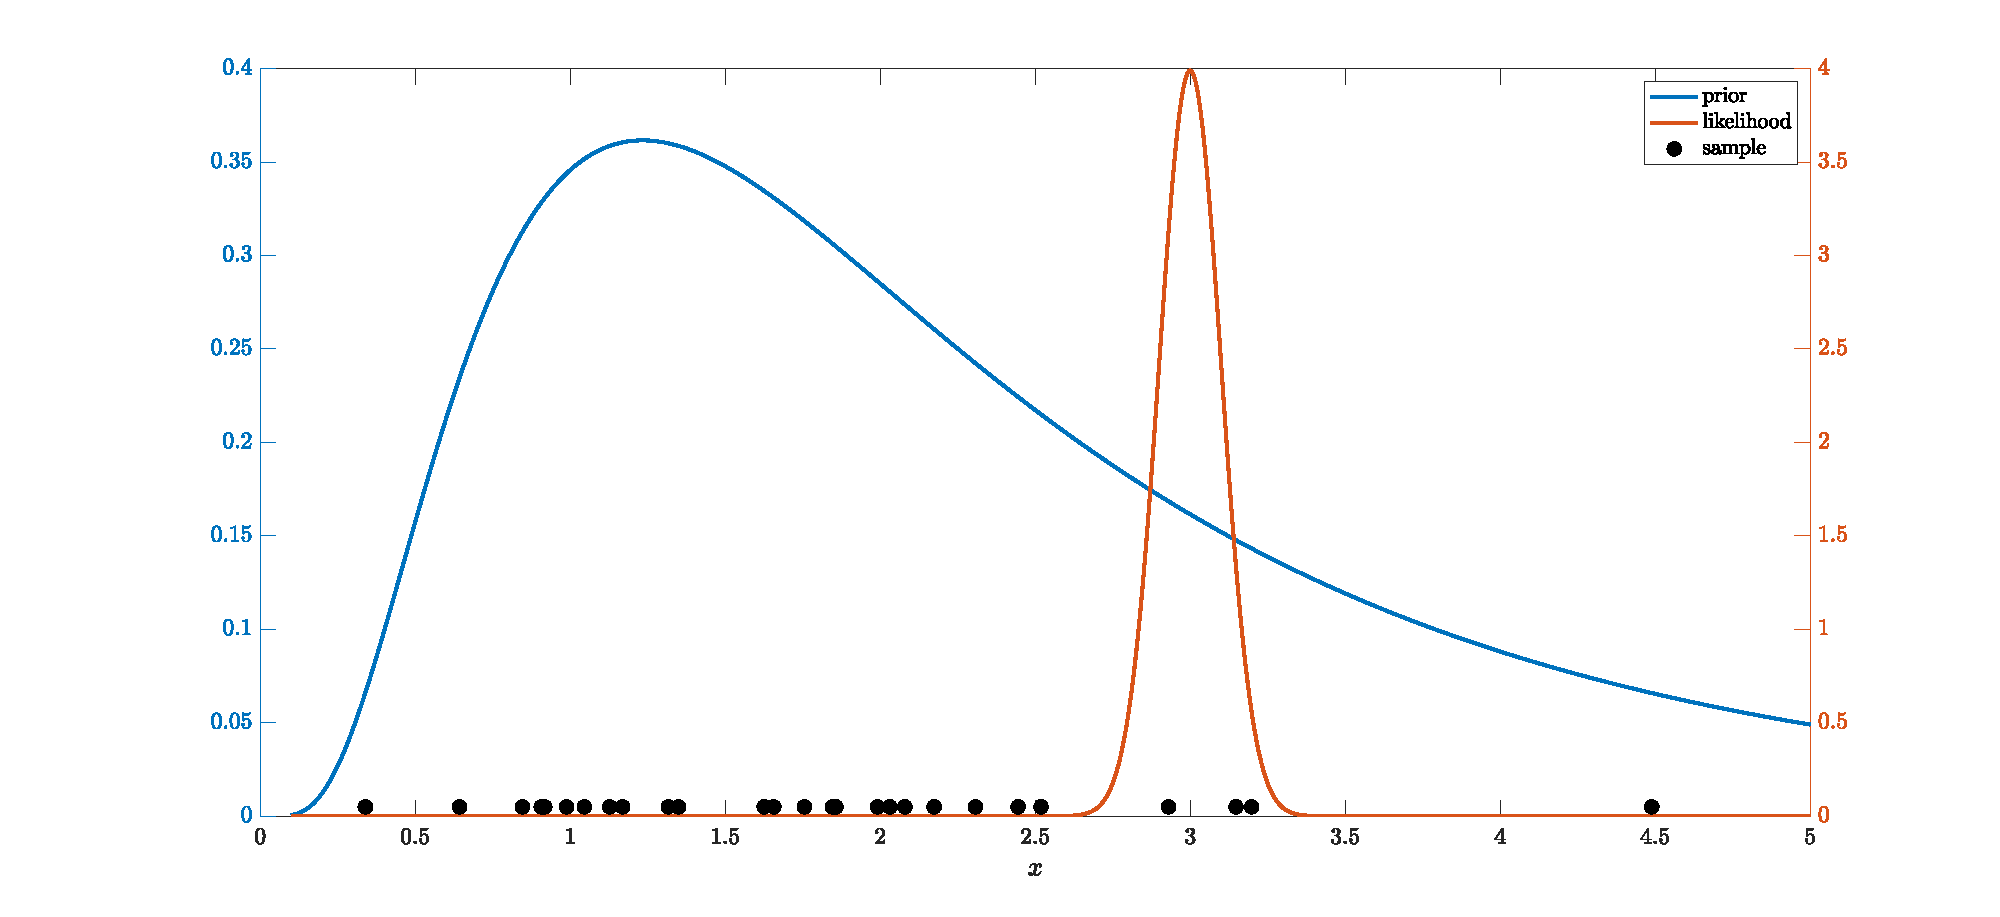
\includegraphics[width = \linewidth]{pf_degen.pdf}
  \caption{Particle degeneracy, shown in a one-dimensional example with 30 particles.}
  \label{fig:pf-degen}
\end{figure}
There are three possible ways to minimalize particle degeneracy: the most obvious one is to have more particles (populate the state space more densely). However, in higher dimensions this demands exponentially more particles. Another solution is to use a different proposal density, therefore having a different likelihood function. In this way the target distribution could be more effectively represented by particles. The third one is resampling: having more particles on top of each other in the same place is better than having only a few of them, while all the others are spread across the domain with negligible weights.


Although particle filters demand low computational power, this only holds when the algorithm is properly tuned, therefore requires the minimal amount of particles. A poor choice of a particle filter, or a poorly designed particle filter requires a lot of computational capacity to give proper results: the particle requirement can be in the order of millions. As were mentioned in \cite{Daum2003}, ``for typical low dimensional tracking problems, the PF requires 2 to 6 orders of magnitude more computer throughput than the extended Kalman filter, to achieve the same accuracy.''

\subsection{The Daum--Huang Filters}
\subsubsection{Main concepts}
To overcome the  undesirable properties of the particle filters (especially the curse of dimensionality), Daum and Huang proposed a new method, where the state estimation is based on a particle flow, induced by a log-homotopy \cite{Daum2007}. This new filtering method is called Daum-Huang filter (DHF) \cite{Choi2011}.

In particle filters, the problem lies where the Bayes' law is performed to obtain the posterior (this is done though weighting). Upon resampling, the particles ``jump'' from the prior to the posterior. The main concept behind the DHF is to eliminate this often faulty ``jump'', and handle it as a continuous movement. Consider a homotopy in $\lambda$, based on the logarithmic form of the Bayes' law:
\begin{equation}\label{eq:bayes-loghom}
  \log p(\mathbf{x},\lambda) = \log g(\mathbf{x}) + \lambda \log h(\mathbf{x}) - \log K(\lambda),
\end{equation}
where $g(\cdot)$ is the prior, $h(\cdot)$ is the likelihood, $K(\cdot)$ is a normalization constant, and $\lambda$ is the parameter of the homotopy: $\lambda \in [0,1]$. As $\lambda$ changes continuously form 0 to 1, $p(\cdot)$ changes from being the prior $g(\cdot)$, to becoming the posterior, as $\lambda = 1$ (this gives back the standard Bayes' rule). This is essentially the time evolution (in this case $\lambda$ is \emph{pseudotime}) of $p(\cdot)$. Meanwhile the particles that represent the probability distribution also have to move: this movement is described by a stochastic law of motion, with $\lambda$ as the time variable. The question is that how to move these particles according to the also evolving probability distribution, from which they were sampled.

It is assumed that the particles are moving according to the following (It\^{o}) stochastic  differential equation:
\begin{equation}\label{eq:dhf-sde}
  \mathrm{d} \mathbf{x}=\mathbf{f}(\mathbf{x}, \lambda) \mathrm{d} \lambda+\boldsymbol{\sigma}(\mathbf{x}, \lambda) \mathrm{d} \mathbf{W}_{\lambda},
\end{equation}
where $\mathbf{f}(\mathbf{x},\lambda)$ is the drift coefficient,
$\boldsymbol\sigma(\mathbf{x},\lambda)$ is the diffusion matrix,
and $\mathbf{W}_\lambda$ denotes the standard Brownian motion (Wiener process) in
pseudotime $\lambda$.

The evolution of a probability density under the governing SDE \eqref{eq:dhf-sde} is described by the Fokker--Planck equation, if $\mathbf{x} \in \mathbb{R}^d$:

\begin{equation}\label{eq:fpe}
  \frac{\partial p(\mathbf{x},\lambda)}{\partial \lambda} = -\sum_{i = 1}^{d}\frac{\partial}{\partial x_i}\left[f_i(\mathbf{x},\lambda)p(\mathbf{x},\lambda)\right] + \frac{1}{2}\sum_{i = 1}^{d}\sum_{j = 1}^{d}\frac{\partial^2}{\partial x_i \partial x_j}\left[B_{i,j}(\mathbf{x},\lambda)p(\mathbf{x},\lambda)\right],
\end{equation}
where
\begin{equation}\label{key}
  \mathbf{B} = \frac{1}{2}\boldsymbol\sigma\boldsymbol\sigma^\top.
\end{equation}
Now if \eqref{eq:bayes-loghom} is partially derivated according to $\lambda$, it can be substituted into the left hand side of \eqref{eq:fpe}. After some simplification, the flow equation in its final form:
\begin{align}\label{eq:dhf-eq}
  \log h(\mathbf{x}) - \frac{\partial \log K(\lambda)}{\partial \lambda} & = -\mathbf{f}^\top(\mathbf{x},\lambda)\cdot\nabla\log p(\mathbf{x},\lambda) - \nabla\cdot \mathbf{f}(\mathbf{x},\lambda)       \\
                                                                         & + \frac{1}{2p(\mathbf{x},\lambda)}\left(\nabla^\top\mathbf{B}(\mathbf{x},\lambda)p(\mathbf{x},\lambda)\nabla\right). \nonumber
\end{align}

\subsubsection{Existing Daum--Huang Filter Variants}
The main difference between the different DHF realizations is the method to solve \eqref{eq:dhf-eq} for $\mathbf{f}(\cdot)$. This is still an open question, and holds much room for innovation even to this day.

Solving \eqref{eq:dhf-eq} requires various simplifications. One approach is the assumption of an exact flow, where the diffusion part is neglected (only deterministic flow is considered), the measurement model is linear (or linearized), and the noise acting on the system is a Gaussian random variable (or from the exponential family). When the linearization of the measurement function is performed around the location of \emph{each} particle instead of their average, the local exact flow Daum--Huang filter is constructed \cite{Ding2012}. Particle weighting can be developed for Daum--Huang filters as well, proposed in \cite{Li2016}.

Another simplification is the assumption of incompressible flow \cite{Daum2007}  (this was the first type of the Daum--Huang filter), the assumption of geodesic flow \cite{Daum2013}, and the latest results are from the consideration of stochastic particle flow (the diffusion term is no longer neglected), using Gromov's method \cite{Daum2018,Dai2021}.
\subsubsection{The Exact Flow Daum--Huang Filter}

Under the criteria, that $g(\mathbf{x})$ and $h(\mathbf{x})$ (the prior and the likelihood, essentially the motion model and the measurement model respectively) are Gaussian,
they can be expressed as:
\begin{align}
  \log g(\mathbf{x}) & =-\frac{1}{2}(\mathbf{x}-\phi(\mathbf{x}',\mathbf{u}',0))^{\top} \mathbf{Q}^{-1}(\mathbf{x}-\phi(\mathbf{x}',\mathbf{u}',0)),            \\
  \log h(\mathbf{x}) & =-\frac{1}{2}(\mathbf{z}'-\psi(\mathbf{x},0))^{\top} \mathbf{R}^{-1}(\mathbf{z}'-\psi(\mathbf{x},0)). \label{eq:explicit-log-likelihood}
\end{align}
Then the solution of \eqref{eq:dhf-eq} has the form of
\begin{equation}\label{eq:edh-flow-vector}
  \mathbf{f}(\mathbf{x},\lambda) = \mathbf{C}(\lambda)\mathbf{x} + \mathbf{c}(\lambda),
\end{equation}
where
\begin{align}
   & \mathbf{C}(\lambda) = -\frac{1}{2}\mathbf{\mathbf{\overline\Sigma}}\nabla \psi_x^\top\left(\lambda \nabla \psi_x\mathbf{\overline\Sigma}\nabla \psi_x^\top + \mathbf{R}\right)^{-1}\nabla \psi_x,\label{eq:edh-C}                              \\
   & \mathbf{c}(\lambda) = \left(\mathbf{I}+2\lambda\mathbf{C}\right)\left[\left(\mathbf{I}+\lambda\mathbf{C}\right)\mathbf{\overline\Sigma}\nabla \psi_x^\top\mathbf{R}^{-1}\mathbf{z}' + \mathbf{C}\overline{\mathbf{x}}\right]. \label{eq:edh-c}
\end{align}
Here, $\overline{\mathbf{x}}$ denotes the state average across all the particles for $\lambda = 0$ at a given timestep,
and $\nabla \psi_x$ is the Jacobian of the measurement function, performed around $\overline{\mathbf{x}}_\lambda$,
which is the particle state average for the given $\lambda$.

By solving for $\mathbf{f}(\mathbf{x},\lambda)$,
the state flow vector is obtained according to \eqref{eq:dhf-sde}.
Recall that for the exact flow simplification, the diffusion term $\boldsymbol\sigma$ is
neglected, resulting
\begin{equation}
  \frac{\mathrm{d}\mathbf{x}}{\mathrm{d}\lambda} = \mathbf{f}(\mathbf{x},\lambda).
\end{equation}
Now the motion of the particles is easily described in pseudotime $\lambda$.

The Exact Flow Daum--Huang Filter (EDH) algorithm is summarized as follows.
In one timestep, first the particles are propagated just like in the case of the PF, then $\overline{\mathbf{\Sigma}}$ is calculated using the prediction part of an EKF/UKF.  After this, the homotopy is discretized: $\lambda$ is equally divided into a certain amount of steps. For each \emph{pseudotime} step, $\nabla \psi_x$ is calculated  by linearization around the current state average of the particles, then using the predicted covariance $\overline{\mathbf{\Sigma}}_t$, the measurement $\mathbf{z}'_t$, the measurement noise covariance $\mathbf{R}_t$, and the state average $\overline{\mathbf{x}}_\lambda$, $\mathbf{C}(\lambda)$ and $\mathbf{c}(\lambda)$ is calculated. By this, the drift function $\mathbf{f}(\cdot)$ is obtained. Now, a simple Euler step yields the new state of the particles. Lastly, $\overline{\mathbf{x}}_\lambda$ is re-evaluated. This is repeated for all $\lambda$. It is important to mention that during the homotopy, the time does not change, only the pseudotime $\lambda$. When $\lambda$ has reached 1, the particles are in the position where they estimate the posterior distribution. Now, the state estimation at $t$ can be calculated by taking the average of the particles. Finally, the EKF/UKF update is performed. This was one time step (and along with it, 10 pseudotime step) of the EDH filter.

Figure \ref{fig:dhf-ill}. illustrates the particle flow of the EDH. The time is fixed, and the homotopy is performed from $\lambda = 0$ to $\lambda = 1$. At $\lambda = 1$, the particles moved from the predicted belief (prior, in this context) to their position where they represent the posterior. The true state is indicated by a red square, while the orange dot is the average of the particles. The red arrows show the value of the drift coefficient $\mathbf{f}(\mathbf{x},\lambda)$. As $\lambda$ evolves, the particle average gets closer and closer to the (unknown) true position.

\begin{figure}
  \centering
  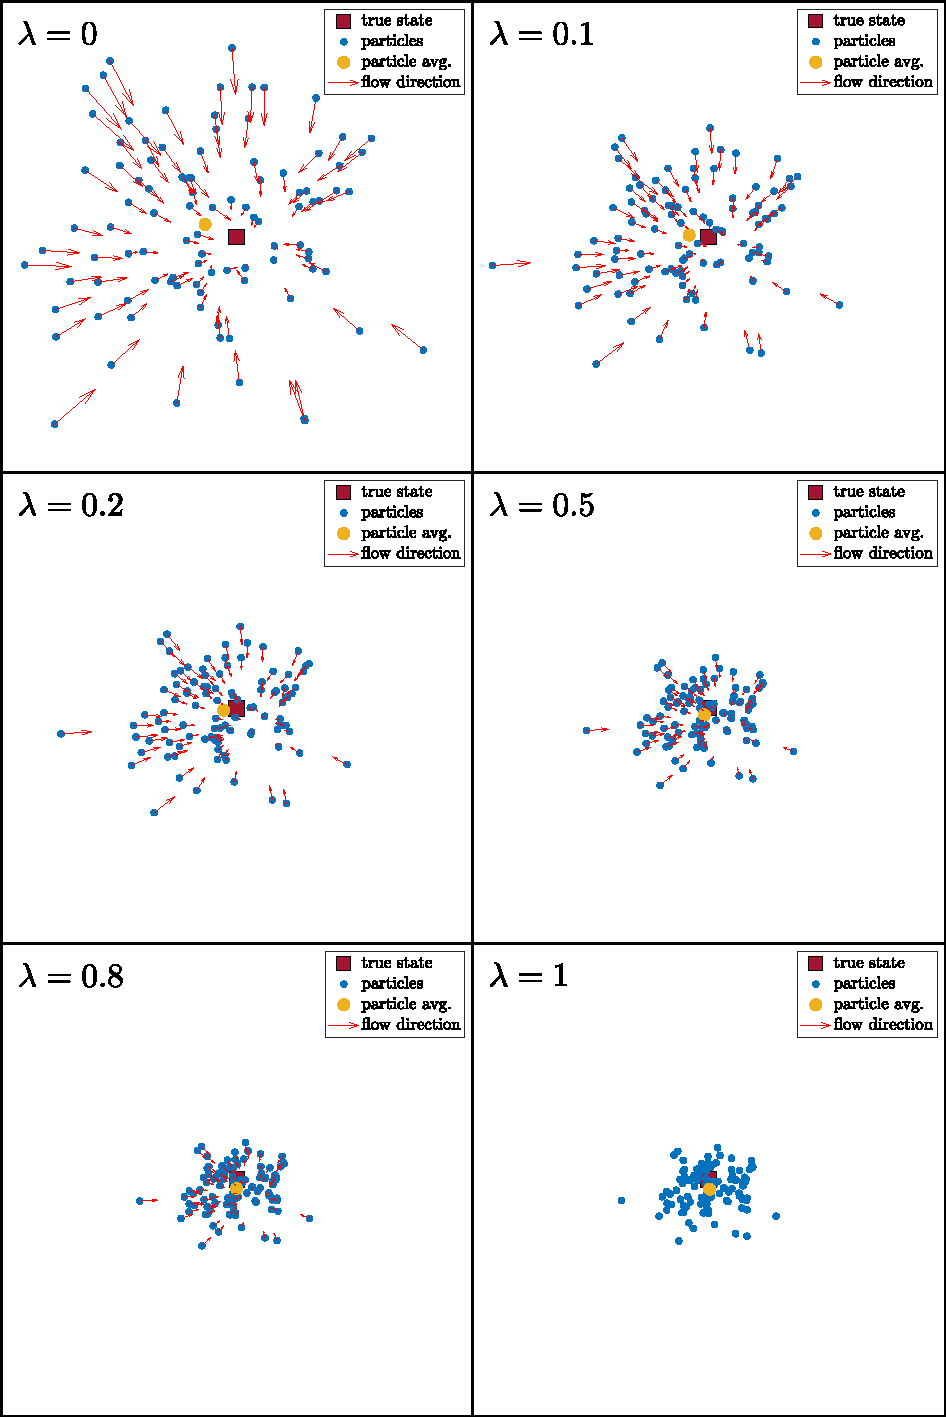
\includegraphics[width=0.98\linewidth]{DHF-visu1.pdf}
  \caption{Particle flow of the EDH. The time is at a fixed value, while the homotopy is performed from $\lambda = 0$ to $\lambda = 1$.}
  \label{fig:dhf-ill}
\end{figure}

\subsubsection{EDH for Implicit Measurement Equation}

Similarly to the case of the EKF, the discussed EDH filter in its original form is not capable of
handling implicit measurement equations.
In \cite{Zhang2012}, the formula for the implicit EKF is derived,
which serves as a foundation for the implicit EDH.

Take the observation function of \eqref{eq:observation-function},
and expand it into a Taylor series about the predicted state, and the measurement for the given timestep: $\left(\overline{\boldsymbol\mu}_t,\mathbf{z}'_t\right)$. This yields
\begin{align}
  \psi(\mathbf{x}_t,\mathbf{z}_t) = \psi(\overline{\boldsymbol\mu}_t,\mathbf{z}'_t)
  + \frac{\partial \psi(\overline{\boldsymbol\mu}_t,\mathbf{z}'_t)}{\partial \mathbf{x}_t}(\mathbf{x}_t-\overline{\boldsymbol\mu}_t)
  + \frac{\partial \psi(\overline{\boldsymbol\mu}_t,\mathbf{z}'_t)}{\partial \mathbf{z}_t}(\mathbf{z}_t-\mathbf{z}'_t) \\
  + \mathcal{O}((\mathbf{x}_t-\overline{\boldsymbol\mu}_t)^2)
  + \mathcal{O}((\mathbf{z}_t-\mathbf{z}'_t)^2) \nonumber.
\end{align}

By neglecting the higher order terms, rearranging the equation, and also using that \linebreak
$\psi(\mathbf{x}_t,\mathbf{z}_t) = 0$:
\begin{align}
   & \frac{\partial \psi(\overline{\boldsymbol\mu}_t,\mathbf{z}'_t)}{\partial \mathbf{x}_t}\overline{\boldsymbol\mu}_t
  - \psi(\overline{\boldsymbol\mu}_t,\mathbf{z}'_t) = \underbrace{\frac{\partial \psi(\overline{\boldsymbol\mu}_t,\mathbf{z}'_t)}{\partial \mathbf{x}_t}}_{\nabla \psi_x}\mathbf{x}_t + \underbrace{\frac{\partial \psi(\overline{\boldsymbol\mu}_t,\mathbf{z}'_t)}{\partial \mathbf{z}_t}}_{\nabla \psi_z}\underbrace{(\mathbf{z}_t-\mathbf{z}'_t)}_{\mathbf{w}_t}, \\
   & \mathbf{y}_t :=  \frac{\partial \psi(\overline{\boldsymbol\mu}_t,\mathbf{z}'_t)}{\partial \mathbf{x}_t}\overline{\boldsymbol\mu}_t
  - \psi(\overline{\boldsymbol\mu}_t,\mathbf{z}'_t) = \nabla\psi_x(\overline{\boldsymbol\mu}_t,\mathbf{z}'_t)\overline{\boldsymbol\mu}_t-\psi(\overline{\boldsymbol\mu}_t,\mathbf{z}'_t) \label{eq:edh-implicit-y}.
\end{align}
As a result, a linear measurement equation is obtained, similarly to \eqref{eq:lin-meas-model}:
\begin{equation}
  \mathbf{y}_t = \nabla \psi_x \mathbf{x}_t + \nabla \psi_z\mathbf{w}_t,\quad\quad \mathbf{w}_t \sim \mathcal{N}(0,\mathbf{R}).
\end{equation}

For this formulated explicit measurement equation, \eqref{eq:explicit-log-likelihood} can be written as
\begin{equation}
  \log h(\mathbf{x}) =-\frac{1}{2}(\mathbf{y}-\nabla \psi_x \mathbf{x}_t)^{\top} (\nabla \psi_z\mathbf{R}\nabla \psi_z^{\top})^{-1}(\mathbf{y}-\nabla \psi_x \mathbf{x}_t).
\end{equation}

Now carrying on with the derivation in \cite{Khan2018} with this modified log-likelihood,
the altered form of \eqref{eq:edh-C} and \eqref{eq:edh-c} for an implicit measurement
equation is:
\begin{align}
   & \mathbf{C}(\lambda) = -\frac{1}{2}\mathbf{\mathbf{\overline\Sigma}}\nabla \psi_x^\top\left(\lambda \nabla \psi_x\mathbf{\overline\Sigma}\nabla \psi_x^\top + \nabla \psi_z\mathbf{R}\nabla \psi_z^{\top}\right)^{-1}\nabla \psi_x,  \label{eq:edh-C-impl}                             \\
   & \mathbf{c}(\lambda) = \left(\mathbf{I}+2\lambda\mathbf{C}\right)\left[\left(\mathbf{I}+\lambda\mathbf{C}\right)\mathbf{\overline\Sigma}\nabla \psi_x^\top(\nabla \psi_z\mathbf{R}\nabla \psi_z^{\top})^{-1}\mathbf{y} + \mathbf{C}\overline{\mathbf{x}}\right]. \label{eq:edh-c-impl}
\end{align}
\subsection{Realization of the EDH for the Inspected Localization Problem}

The original EDH algorithm for implicit measurement equation is described
in \cite{Ding2012}.
Now, that the implicit EDH is introduced along with the motion and measurement models
for the localization problem in scope, the full algorithm for the EDH can be formulated.
Algorithm \ref{alg:edh-loc}. contains one step of the filter.
For each computation, the relevant equations are indicated at the end of the line.
The resulting estimated state is $\overline{\mathbf{x}}_t$, which is then used to evaluate the performance of the proposed method in the next section.
\begin{algorithm}
  \caption{Exact Flow Daum--Huang Filter for Localization($\boldsymbol{\mu}_{t-1},\mathbf{\Sigma}_{t-1},\hat{\mathbf{u}}_t,\mathbf{z}'_t,\{\mathbf{x}_t^i\}_{i=1}^{N}$)}\label{alg:edh-loc}
  \begin{algorithmic}[1]
    \If{t is 0} \Comment{initialization step}
    \State Draw $N$ particles from a prior distribution: $\{\mathbf{x}_0^i\}_{i=1}^{N}$;
    \State Calc. the mean $\boldsymbol\mu_0$ and covar. $\boldsymbol\Sigma_0$ of the particle set, assign $\overline{\mathbf{x}}_0 = \boldsymbol{\mathbf{\mu}}_0$;
    \State\Return $\boldsymbol{\mu}_0,\boldsymbol{\Sigma}_0,\{\mathbf{x}_0^i\}_{i=1}^{N},\overline{\mathbf{x}}_0$;
    \EndIf
    \State Calculate $\mathbf{u}_t$, using $\hat{\mathbf{u}}_t$; \Comment{\eqref{eq:odom-raw-input}-\eqref{eq:odom-delta-input}}
    \State Calculate $\mathbf{Q}_t$ using $\mathbf{u}_t$
    \Comment{\eqref{eq:control-covar}}
    \State Propagate particles: $\mathbf{x}_t^{i} = \phi(\mathbf{x}_{t-1}^{i},\mathbf{u}_t,\mathbf{v}_t)$;
    \Comment{\eqref{eq:prop-x}-\eqref{eq:prop-theta}}
    \State Calculate the average of the particle set $\{\mathbf{x}_t^i\}_{i=1}^{N}$: $\overline{\mathbf{x}}_t$;
    \State Assign $\overline{{\mathbf{x}}}_{t,0} = \overline{\mathbf{x}}_t$;
    \State EKF prediction:
    \State\indent Evaluate the Jacobians at $(\boldsymbol{\mu}_{t-1},\mathbf{u}_t)$:
    \Comment{\eqref{eq:motmodel-jacobi-x}-\eqref{eq:motmodel-jacobi-u}}
    \State\indent\indent $\nabla\phi_x := \nabla\phi_x(\boldsymbol{\mu}_{t-1},\mathbf{u}_t),\quad \nabla\phi_u := \nabla\phi_x(\boldsymbol{\mu}_{t-1},\mathbf{u}_t)$;
    \State\indent$\overline{\boldsymbol{\mu}}_t = \phi(\boldsymbol{\mu}_{t-1},\mathbf{u}_t,\mathbf{v}_t = 0)$;
    \State\indent
    $\overline{\mathbf{\Sigma}}_t = \nabla \phi_x\mathbf{\Sigma}_{t-1}\nabla \phi_x^{\top}
      +\nabla \phi _u\mathbf{Q}_t \nabla \phi_u^{\top}$;
    \For{$j = 1\dots N_{\lambda}$} \Comment{$N_{\lambda}:$ number of $\lambda$ steps}
    \State $\lambda = j\Delta\lambda$;
    \Comment{$\Delta\lambda$: step size}
    \State Evaluate $\nabla\psi_x(\overline{\mathbf{x}}_t,\mathbf{z}'_t),\nabla\psi_z(\overline{\mathbf{x}}_t,\mathbf{z}'_t)$;
    \Comment{\eqref{eq:measmodel-jacobi-x}-\eqref{eq:measmodel-jacobi-z}}
    \State Calculate $\mathbf{y}_t$, using $\overline{\mathbf{x}}_t,\mathbf{z}'_t$,$\nabla\psi(\overline{\mathbf{x}}_t,\mathbf{z}'_t)$; \Comment{\eqref{eq:edh-implicit-y},\eqref{eq:observation-function}}
    \State Calculate $\mathbf{C}$ and $\mathbf{c}$, using
    $\lambda,\overline{\boldsymbol\Sigma}_t, \overline{\mathbf{x}}_{t,0}$,
    $\nabla\psi_x(\overline{\mathbf{x}}_t,\mathbf{z}'_t),\nabla\psi_z(\overline{\mathbf{x}}_t,\mathbf{z}'_t), \mathbf{y}_t$;
    \Comment{\eqref{eq:edh-C-impl}-\eqref{eq:edh-c-impl}}
    \State Evaluate $\mathbf{f}(\mathbf{x},\lambda)$ for every particle $\mathbf{x}_t^{i}$, resulting $\frac{\mathrm{d}\mathbf{x}_t^i}{\mathrm{d}\lambda}$;
    \Comment{\eqref{eq:edh-flow-vector}}
    \State Update the pose of each particle by an Euler-step:
    \State\indent $\mathbf{x}_t^{i} = \mathbf{x}_t^{i} + \Delta\lambda\frac{\mathrm{d}\mathbf{x}_t^i}{\mathrm{d}\lambda}$;
    \State Re-evaluate $\overline{\mathbf{x}}_t$ with the updated particle poses;
    \EndFor
    \State EKF update:
    \State\indent Evaluate the Jacobians at $(\overline{\boldsymbol{\mu}}_t,\mathbf{z}'_t)$:
    \Comment{\eqref{eq:motmodel-jacobi-x}-\eqref{eq:motmodel-jacobi-u}}
    \State\indent\indent $\nabla\psi_x := \nabla\psi_x(\overline{\boldsymbol{\mu}}_t,\mathbf{z}'_t), \quad \nabla\psi_z := \nabla\psi_z(\overline{\boldsymbol{\mu}}_t,\mathbf{z}'_t)$;
    \State\indent $\mathbf{K}_t = \overline{\mathbf{\Sigma}}_t\nabla \psi_x^\top\left(\nabla \psi_x\overline{\mathbf{\Sigma}}_t\nabla \psi_z^\top+
      \nabla \psi_z\mathbf{R}\nabla \psi^{\top}_z\right)^{-1}$;
    \State\indent $\boldsymbol{\mu}_t = \overline{\boldsymbol{\mu}}_t + \mathbf{K}_t\left(0-\psi(\overline{\boldsymbol{\mu}}_t,\mathbf{z}'_t)\right)$;
    \Comment{\eqref{eq:observation-function}}
    \State\indent $\mathbf{\Sigma}_t = \left(\mathbf{I}-\mathbf{K}_t\nabla \psi_x\right)\overline{\mathbf{\Sigma}}_t$;
    \State\Return $\boldsymbol{\mu}_t,\boldsymbol{\Sigma}_t,\{\mathbf{x}_t^i\}_{i=1}^{N},\overline{\mathbf{x}}_t$;
  \end{algorithmic}
\end{algorithm}

\pagebreak
\section{Evaluation of the Proposed EDH Localization Algorithm}
\subsection{Experimental Setup}

In the following, the performance of three localization algorithms is going to be compared:
the EKF-based localization  by Dantanarayana et al. \cite{Dantanarayana2016},
the EDH-based localization  algorithm proposed in this report,
and the Adaptive Monte Carlo Localization (AMCL) in ROS \cite{AMCLROS2002}.
For the sake of simplicity, the EDH-based, and the EKF-based
algorithms are going to be referred by their underlying filter (EDH and EKF).

To evaluate the algorithms, simulational data is provided by the Gazebo
simulator, where the TurtleBot3 robot is placed inside the TurtleBot3 House
(see Subsection \ref{subsec:robot} and \ref{subsec:map} for more details).

For one simulational run, the agent is driven around in the environment by hand.
Meanwhile, the AMCL runs in the background, and performs the localization.
The other two methods are not implemented in ROS, therefore require the
simulation data to be exported from Gazebo.
Upon the evaluation of the EKF and the EDH, this data is imported
from an external file, simulating real-time measurements.
This file contains the LiDAR measurements, the pose of the robot obtained
by odometry,
the ground truth pose, and the pose estimation by AMCL.

For AMCL, the default parameters are used, provided by ROBOTIS \footnote{https://github.com/ROBOTIS-GIT/turtlebot3}.
The initial mean of the EKF is the exact starting pose of the robot, and the
covariance is
\begin{equation}
    \boldsymbol\Sigma_0 = \text{diag}(\Sigma_{11},\Sigma_{22},\Sigma_{33}),
\end{equation}
where $\Sigma_{11} = 0.1^2\,\text{m}^2$,
$\Sigma_{22} = 0.1^2\,\text{m}^2$,$\Sigma_{33} = 0.05^2\,\text{rad}^2$.

The particles of the EDH are drawn from a prior with mean of the starting pose,
and covariance of $\boldsymbol\Sigma_0$.
For the homotopy, $N_\lambda$ = 10 steps are used, with $\Delta\lambda = 0.1$ as step size.

During different simulational runs, the particle number of the EDH,
and the odometry error constant $\kappa$ from \eqref{eq:odom-noise1} are varied.
\pagebreak
\subsection{Results}
Table \ref{tab:results}. contains the Root Mean Squared Error (RMSE) and Mean Absolute Error (MAE)
of the position and the orientation for different scenarios, using the ground truth pose data
from the simulator. The robustness of the algorithms are tested based on increasing odometry
noise by simulating with $\kappa = \{10^{-6},10^{-4},5\cdot10^{-3}\}$, producing three datasets.

For $\kappa = 10^{-4}$, the estimated trajectories by the filters are plotted in Figure \ref{fig:filtered-traj}.
(All three datasets have a similar ground truth path.) For this same simulation, the
estimation errors for each component of the pose are plotted
in Figures \ref{fig:setup2-x-error}-\ref{fig:setup2-th-error}.

By looking at these figures and the corresponding estimation errors in
Table \ref{tab:results} (rows 5-7), the superiority of the EKF and EDH based
localization algorithms are easily noticeable.
Moreover, the proposed EDH-based algorithm has the least amount of position error, and has only
slightly more orientation error than the EKF.
For less odometry noise ($\kappa = 10^6$), this difference disappears, and the three algorithm
produce similar results.

As $\kappa$ is increased, the position estimation advantage of the EDH algorithm becomes clearer,
although the EKF produces better orientation estimation. An important addition is that increasing
the particle number of the EDH does not yield a better result.

By comparing the estimation errors of the EKF and the EDH in Figure \ref{fig:setup2-x-error},
a beneficial property of the EDH is detectable.
Their error curves are broadly similar, but the EDH produces a less peaked
result, as it almost acts as a low-pass filter. The introduction of the log-homotopy,
and the averaging of the multiple tracked pose hypotheses (the particles)
are mainly responsible for this effect.

The main drawback of the AMCL algorithm lies in its poor performance of estimating
the orientation.  For $\kappa = 10^{-4}$, its position RMSE is twice than of the EDH,
but its orientation RMSE is 3.5 times higher.
Altogether, it is especially sensitive for the increasing odometry noise,
thus producing a 10 times higher RMSE than the EDH at $\kappa = 5\cdot10^{-3}$.

Generally, all of the algorithms performed well in the inspected scenarios, and
did not yield divergent results, even in the case of highly uncertain odometry data.
Inspecting the position errors, the EDH produced the lowest position errors in
all three runs, despite it only required 10 particles to do so.

Regarding computation time, the EKF took 0.52 s for a simulated movement of 429 s,
while the EDH took 40.4 s (running on an Apple M1 ARM with 8 GB of RAM
in Python 3.9).
Although this number is significantly higher
than in the case of the EKF, the main goal was the ability for the proposed
filter to be able to run in real time, which is fulfilled.
There are much room for improvement in in this field, as now the
subject of attention was on the realization of the proposed algorithm itself.
As the EDH operates with multiple particles, a significant improvement could
be achieved by the utilization of multiple CPU cores (making the computations
parallel).
\begin{figure}[htbp]
    \centering
    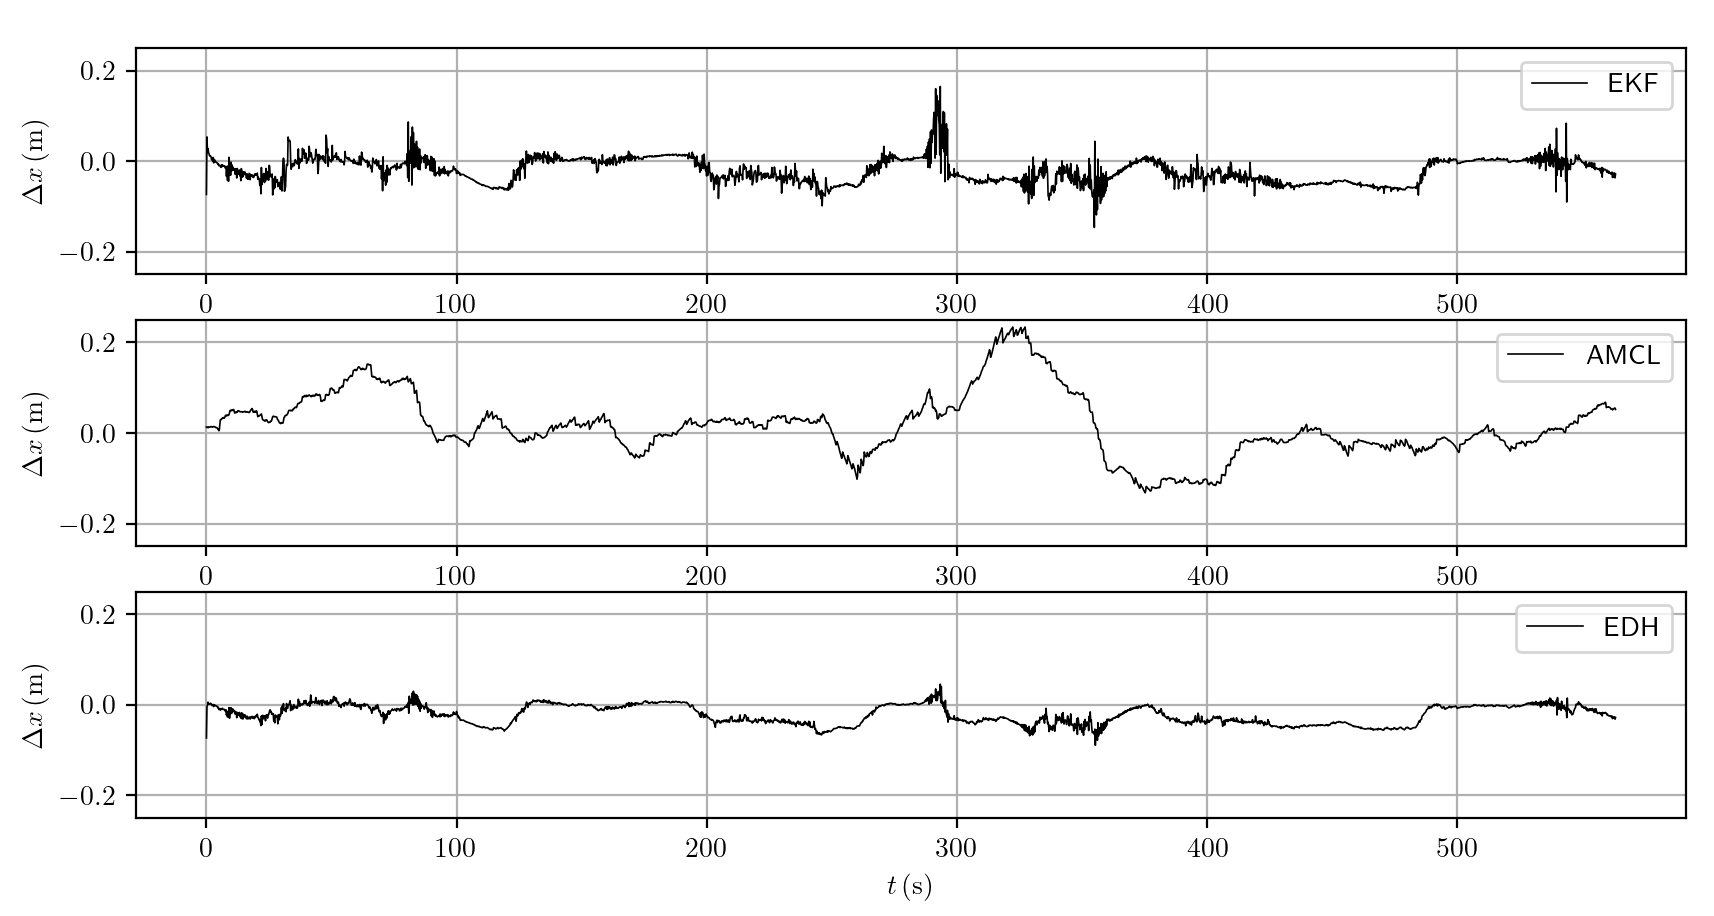
\includegraphics[width=\linewidth]{track_error_x.png}
    \caption{Position error against the ground truth in the $x$ component of the pose vector,
        using the dataset with $\kappa = 10^{-4}$.}
    \label{fig:setup2-x-error}
\end{figure}
\begin{figure}[htbp]
    \centering
    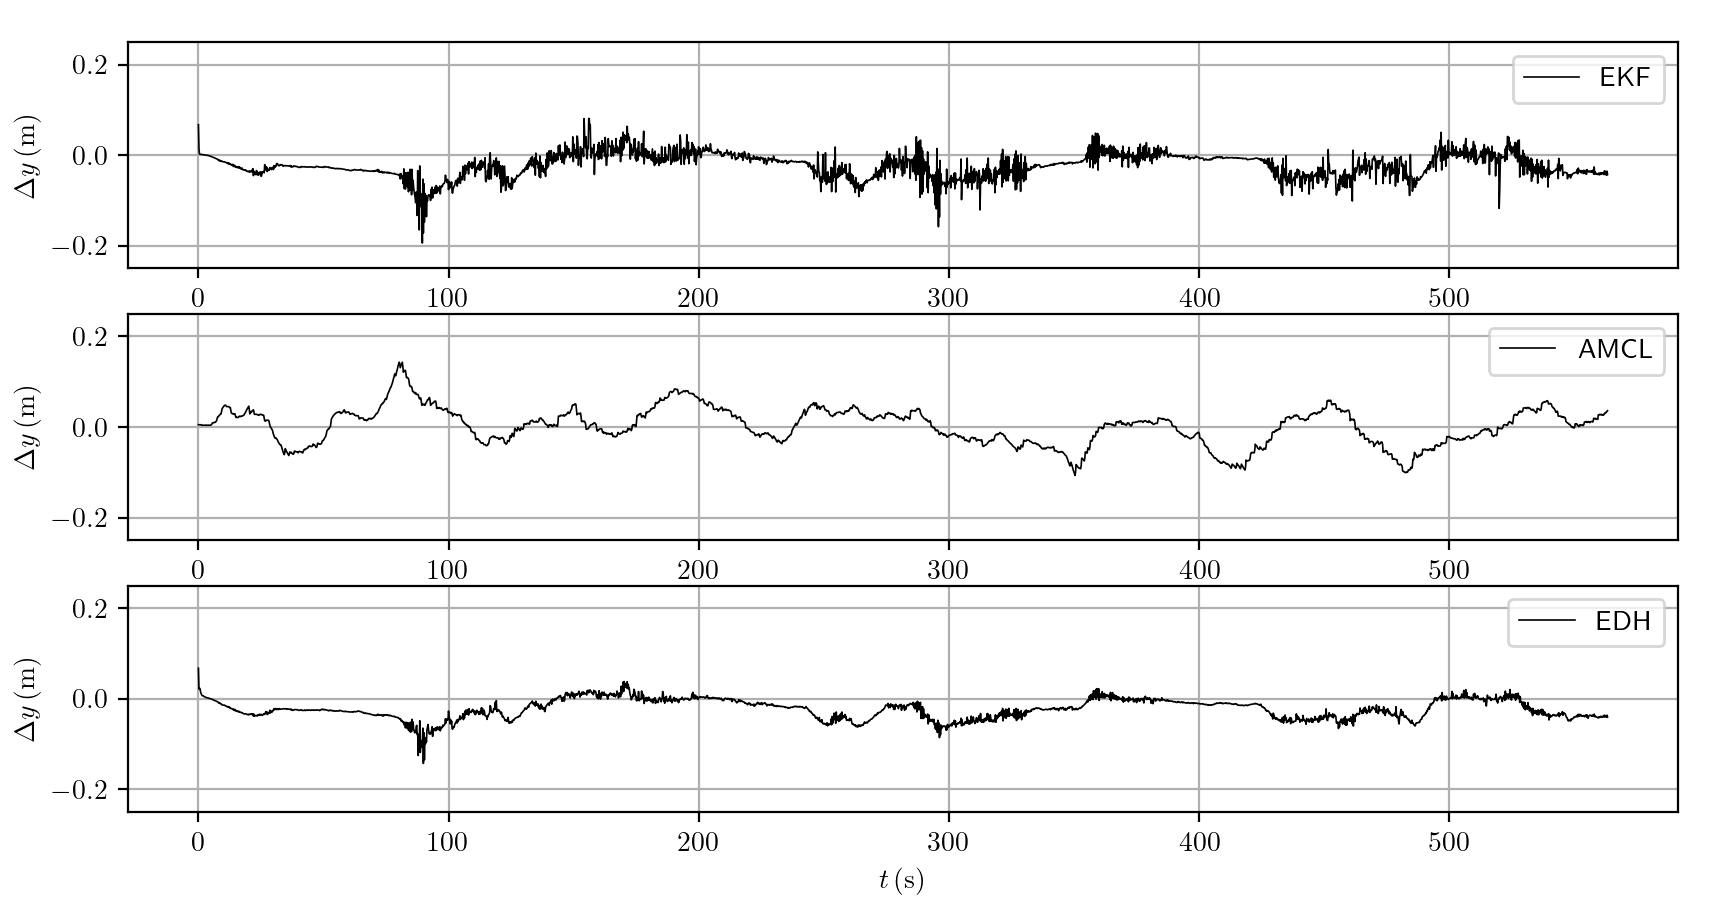
\includegraphics[width=\linewidth]{track_error_y.png}
    \caption{Position error against the ground truth in the $y$ component of the pose vector,
        using the dataset dataset with $\kappa = 10^{-4}$.}
    \label{fig:setup2-y-error}
\end{figure}
\begin{figure}[htbp]
    \centering
    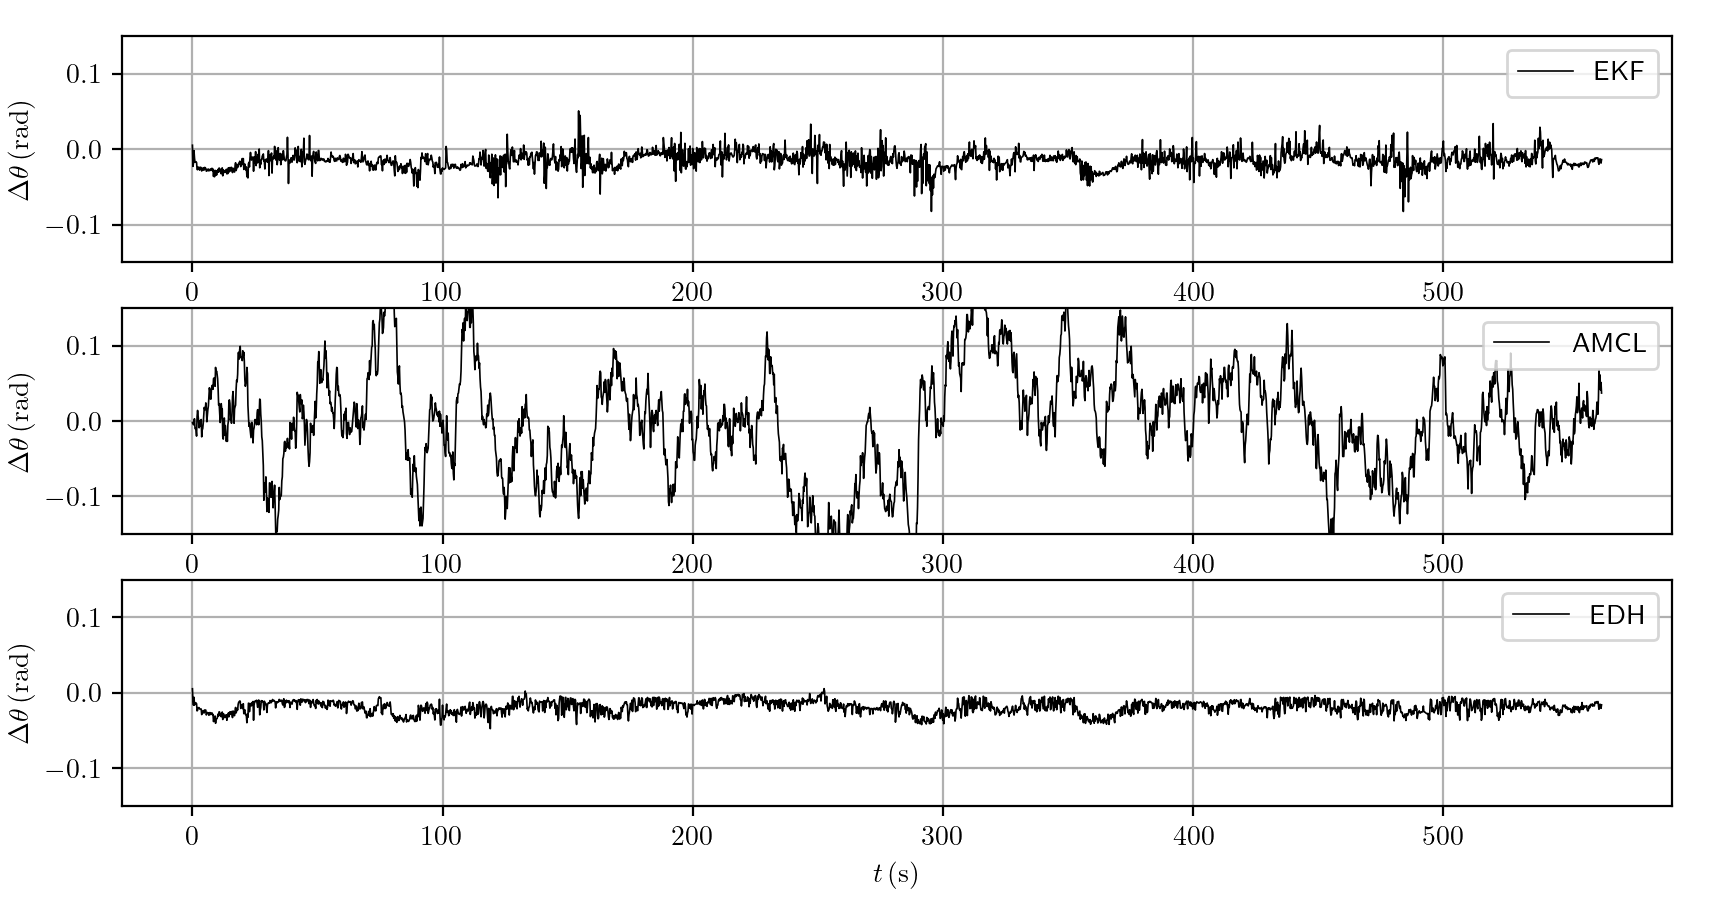
\includegraphics[width=\linewidth]{track_error_th.png}
    \caption{Orientation error against the ground truth in the $\theta$ component of the pose vector,
        using the  dataset with $\kappa = 10^{-4}$.}
    \label{fig:setup2-th-error}
\end{figure}
\begin{table}[]
    \centering
    \begin{tabular}{lllllll}
        \hline
        \multicolumn{1}{|c|}{\multirow{2}{*}{Algorithm}} & \multicolumn{1}{c|}{\multirow{2}{*}{\begin{tabular}[c]{@{}c@{}}$\kappa$\\(m)\end{tabular}}} & \multicolumn{1}{c|}{\multirow{2}{*}{\begin{tabular}[c]{@{}c@{}}Particle\\num.\end{tabular}}} & \multicolumn{2}{c|}{Root Mean Squared Error}   & \multicolumn{2}{c|}{Mean Absolute Error}                                                                                                          \\\cline{4-7}
        \multicolumn{1}{|c|}{}                           & \multicolumn{1}{c|}{}                                           & \multicolumn{1}{c|}{}                                           & \multicolumn{1}{l|}{\begin{tabular}[c]{@{}c@{}}position\\ (m)\end{tabular}} & \multicolumn{1}{c|}{\begin{tabular}[c]{@{}c@{}}orientation\\ (rad)\end{tabular}} & \multicolumn{1}{l|}{\begin{tabular}[c]{@{}c@{}}position\\ ($\text{m}$)\end{tabular}} & \multicolumn{1}{l|}{\begin{tabular}[c]{@{}c@{}}orientation\\ ($\text{rad}$)\end{tabular}} \\ \hline
        \hline
        \multicolumn{1}{|l|}{EKF}                        & \multicolumn{1}{c|}{$10^{-6}$}                                  & \multicolumn{1}{c|}{-}                                          & \multicolumn{1}{c|}{0.0559}                    & \multicolumn{1}{c|}{\textbf{0.0212}}           & \multicolumn{1}{c|}{0.0492}                    & \multicolumn{1}{c|}{\textbf{0.0168}}            \\ \hline
        \multicolumn{1}{|l|}{AMCL}                       & \multicolumn{1}{c|}{$10^{-6}$}                                  & \multicolumn{1}{c|}{adaptive}                                   & \multicolumn{1}{c|}{0.0529}                    & \multicolumn{1}{c|}{0.0233}                    & \multicolumn{1}{c|}{0.0453}                    & \multicolumn{1}{c|}{0.0177}                     \\ \hline
        \multicolumn{1}{|l|}{\multirow{3}{*}{EDH}}       & \multicolumn{1}{c|}{\multirow{3}{*}{$10^{-6}$}}                 & \multicolumn{1}{c|}{10}                                         & \multicolumn{1}{c|}{0.0504}                    & \multicolumn{1}{c|}{0.0228}                    & \multicolumn{1}{c|}{0.0449}                    & \multicolumn{1}{c|}{0.0183}                     \\ \cline{3-7}
        \multicolumn{1}{|l|}{}                           & \multicolumn{1}{c|}{}                                           & \multicolumn{1}{c|}{100}                                        & \multicolumn{1}{c|}{0.0504}                    & \multicolumn{1}{c|}{0.0229}                    & \multicolumn{1}{c|}{0.0447}                    & \multicolumn{1}{c|}{0.0183}                     \\ \cline{3-7}
        \multicolumn{1}{|l|}{}                           & \multicolumn{1}{c|}{}                                           & \multicolumn{1}{c|}{500}                                        & \multicolumn{1}{c|}{\textbf{0.0498}}           & \multicolumn{1}{c|}{0.0231}                    & \multicolumn{1}{c|}{\textbf{0.0441}}           & \multicolumn{1}{c|}{0.0185}                     \\ \hline
        \hline
        \multicolumn{1}{|l|}{EKF}                        & \multicolumn{1}{c|}{$10^{-4}$}                                  & \multicolumn{1}{c|}{-}                                          & \multicolumn{1}{c|}{0.0497}                    & \multicolumn{1}{c|}{\textbf{0.0186}}           & \multicolumn{1}{c|}{0.0428}                    & \multicolumn{1}{c|}{\textbf{0.0159}}            \\ \hline
        \multicolumn{1}{|l|}{AMCL}                       & \multicolumn{1}{c|}{$10^{-4}$}                                  & \multicolumn{1}{c|}{adaptive}                                   & \multicolumn{1}{c|}{0.0816}                    & \multicolumn{1}{c|}{0.0708}                    & \multicolumn{1}{c|}{0.0672}                    & \multicolumn{1}{c|}{0.0547}                     \\ \hline
        \multicolumn{1}{|l|}{\multirow{3}{*}{EDH}}       & \multicolumn{1}{c|}{\multirow{3}{*}{$10^{-4}$}}                 & \multicolumn{1}{c|}{10}                                         & \multicolumn{1}{c|}{0.0439}                    & \multicolumn{1}{c|}{0.0205}                    & \multicolumn{1}{c|}{\textbf{0.0381}}           & \multicolumn{1}{c|}{0.0188}                     \\ \cline{3-7}
        \multicolumn{1}{|l|}{}                           & \multicolumn{1}{c|}{}                                           & \multicolumn{1}{c|}{100}                                        & \multicolumn{1}{c|}{\textbf{0.0437}}           & \multicolumn{1}{c|}{0.0206}                    & \multicolumn{1}{c|}{0.0383}                    & \multicolumn{1}{c|}{0.0190}                     \\ \cline{3-7}
        \multicolumn{1}{|l|}{}                           & \multicolumn{1}{c|}{}                                           & \multicolumn{1}{c|}{500}                                        & \multicolumn{1}{c|}{0.0438}                    & \multicolumn{1}{c|}{0.0206}                    & \multicolumn{1}{c|}{0.0382}                    & \multicolumn{1}{c|}{0.0190}                     \\ \hline
        \hline
        \multicolumn{1}{|l|}{EKF}                        & \multicolumn{1}{c|}{$5\cdot10^{-3}$}                            & \multicolumn{1}{c|}{-}                                          & \multicolumn{1}{c|}{0.0732}                    & \multicolumn{1}{c|}{\textbf{0.0297}}           & \multicolumn{1}{c|}{0.0610}                    & \multicolumn{1}{c|}{\textbf{0.0256}}            \\ \hline
        \multicolumn{1}{|l|}{AMCL}                       & \multicolumn{1}{c|}{$5\cdot10^{-3}$}                            & \multicolumn{1}{c|}{adaptive}                                   & \multicolumn{1}{c|}{0.5261}                    & \multicolumn{1}{c|}{0.4940}                    & \multicolumn{1}{c|}{0.3533}                    & \multicolumn{1}{c|}{0.3841}                     \\ \hline
        \multicolumn{1}{|l|}{\multirow{3}{*}{EDH}}       & \multicolumn{1}{c|}{\multirow{3}{*}{$5\cdot10^{-3}$}}           & \multicolumn{1}{c|}{10}                                         & \multicolumn{1}{c|}{\textbf{0.0587}}           & \multicolumn{1}{c|}{0.0401}                    & \multicolumn{1}{c|}{\textbf{0.0494}}           & \multicolumn{1}{c|}{0.0372}                     \\ \cline{3-7}
        \multicolumn{1}{|l|}{}                           & \multicolumn{1}{c|}{}                                           & \multicolumn{1}{c|}{100}                                        & \multicolumn{1}{c|}{0.0616}                    & \multicolumn{1}{c|}{0.0403}                    & \multicolumn{1}{c|}{0.0503}                    & \multicolumn{1}{c|}{0.0374}                     \\ \cline{3-7}
        \multicolumn{1}{|l|}{}                           & \multicolumn{1}{c|}{}                                           & \multicolumn{1}{c|}{500}                                        & \multicolumn{1}{c|}{0.0617}                    & \multicolumn{1}{c|}{0.0402}                    & \multicolumn{1}{c|}{0.0503}                    & \multicolumn{1}{c|}{0.0373}                     \\ \hline
        \hline
    \end{tabular}
    \caption{Estimation errors of the three filters on three distinct dataset, with increasing odometry error $\kappa$.
        The best results are indicated by bold font for each dataset and each category.}
    \label{tab:results}
\end{table}

\begin{figure}[htbp]
    \centering
    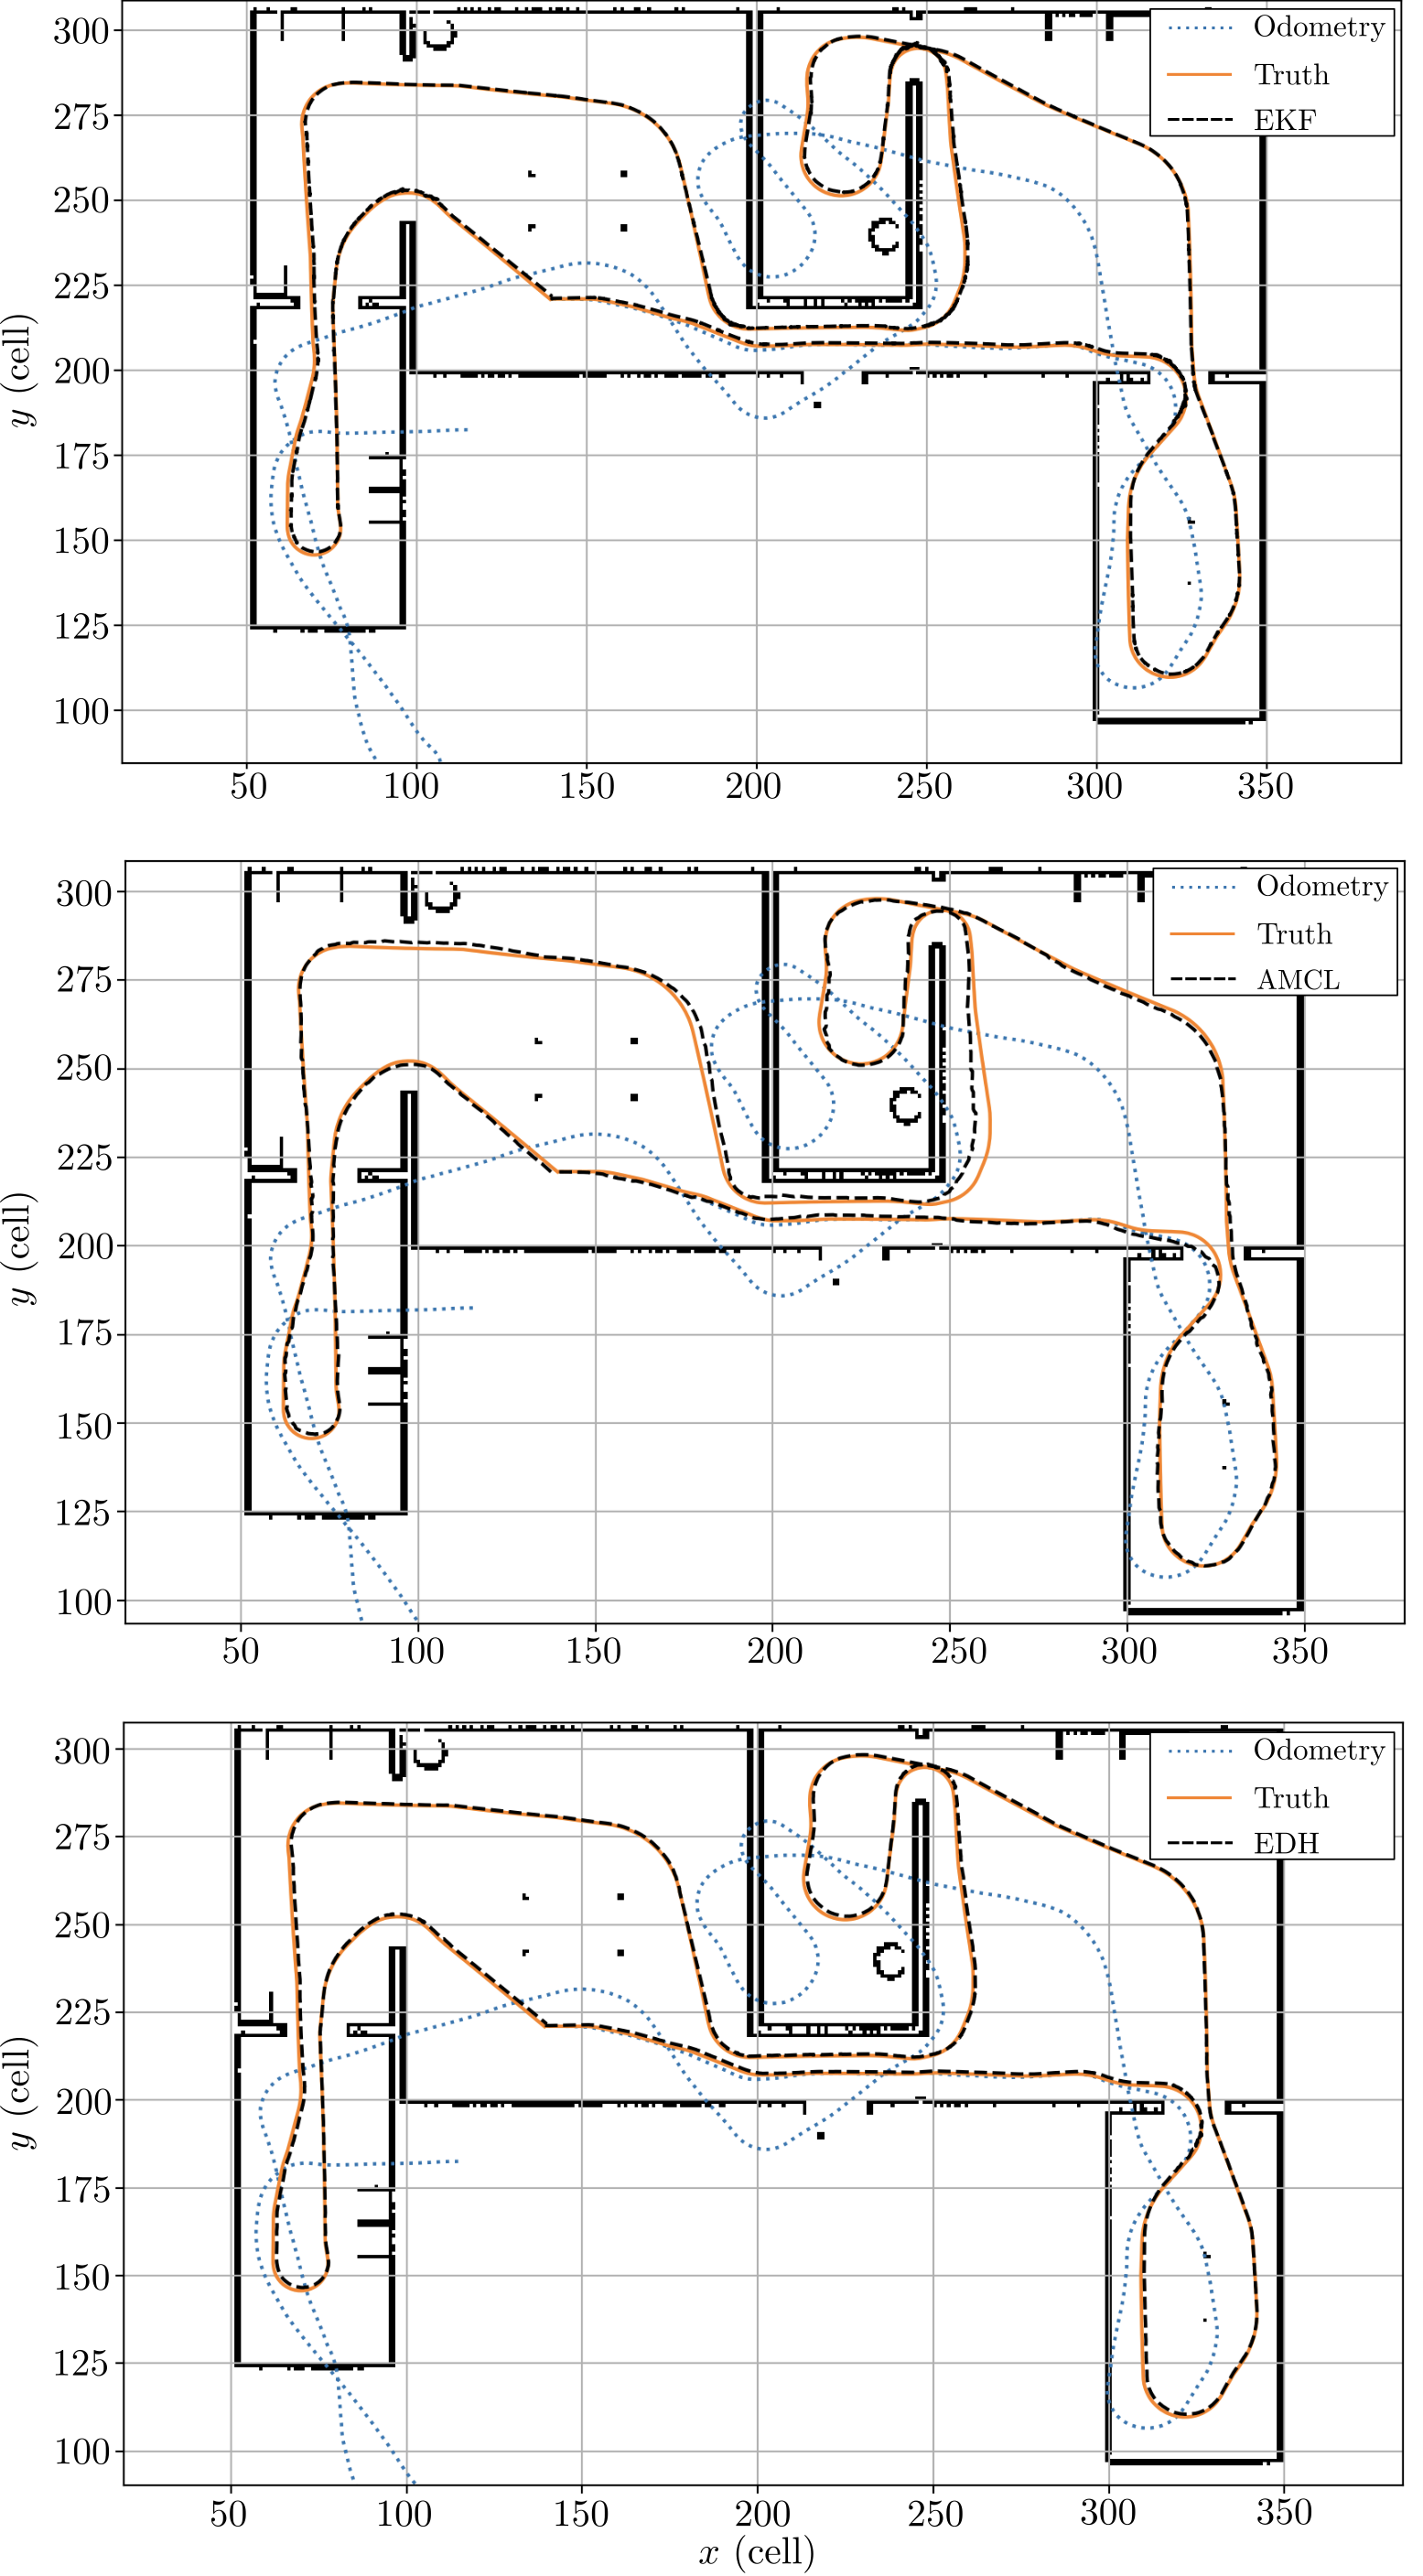
\includegraphics{filtered-tracks.png}
    \caption{Estimated trajectories by the three localization algorithms for $\kappa = 10^{-4}$.}
    \label{fig:filtered-traj}
\end{figure}

\pagebreak
\section{Summary}
During the course of this document, all of the prerequisites for a mobile robot localization were
discussed: the Bayes filter as a foundation,
the motion and the measurement models based on the
sensors and the kinematics of the actual robot,
the representation of the environment as an OGM and
different state estimation algorithms.
First, the extended Kalman filter, followed by the bootstrap particle filter and the exact
flow Daum–Huang filter. Each of them are based on the standard Bayesian state
estimation framework, but provide different approach to handle its update step.
The Kalman filter handles this by the calculation of the Kalman gain and the parametric
approach to describe a Gaussian distribution. Particle filters are much more versatile,
enabling the estimation of multimodal, non-Gaussian probability distributions. The main
drawback of particle filters is the problem of particle degeneracy, and therefore the curse
of dimensionality. To overcome this phenomenon, Daum and Huang proposed a new
method, where a particle flow is used to efficiently move particles from their position in
the prior, to the posterior. This replaced the inefficient resample method of the particle
filter. The flow is described by a partial differential equation, whose solution is required.
This creates a fairly complex theoretical background for the new filter. However, under
certain assumptions the flow can be easily solved, resulting for example in the exact flow
Daum–Huang filter (besides other realizations).
This whole new family of filters carry great potential, and much room for further research
and improvements.

In order to test the beneficial properties the the Daum–Huang filter, a mobile robot
localization algorithm were proposed, which operates on an Occupancy Grid Map, using
LiDAR measurements. The main goal was to make such an algorithm, which is
performance-wise comparable to the popular AMCL algorithm, and the newly proposed EKF-based
algorithm in \cite{Dantanarayana2016}.
This requirement was fulfilled, as the implemented EDH-based localization method
yielded the best (in term of RMSE) position estimation of the three, for all of the
inspected scenarios. It performed well even with highly uncertain odometry source,
where the AMCL resulted in a significantly poorer estimation.

A major area for improving is the computational time, as the proposed algorithm is noticeably
slower than the other two, although it still capable of real-time localization.
In the future, this algorithm will be further developed.
An interesting addition is the particle weighting method from \cite{Li2016}, the localized
particle flow from \cite{Ding2012}, and the introduction of stochastic movement in \cite{Dai2021}.
The main challenge is to develop algorithms and variations that do not require significantly
more computation, yet result in a more robust and more precise estimation of the
state. Besides pure localization, another utmost exciting area is the
the Simultaneous Localization and Mapping task, which is considered as one of the
hardest problem to be solved by a state estimation algorithm. Based on the results
of this report, the Daum--Huang filter could be a promising contender.


\pagebreak
\bibliography{library}

\end{document}
